% Options for packages loaded elsewhere
\PassOptionsToPackage{unicode}{hyperref}
\PassOptionsToPackage{hyphens}{url}
\PassOptionsToPackage{dvipsnames,svgnames,x11names}{xcolor}
%
\documentclass[
  ignorenonframetext,
  aspectratio=169]{beamer}
\usepackage{pgfpages}
\setbeamertemplate{caption}[numbered]
\setbeamertemplate{caption label separator}{: }
\setbeamercolor{caption name}{fg=normal text.fg}
\beamertemplatenavigationsymbolsempty
% Prevent slide breaks in the middle of a paragraph
\widowpenalties 1 10000
\raggedbottom
\setbeamertemplate{part page}{
  \centering
  \begin{beamercolorbox}[sep=16pt,center]{part title}
    \usebeamerfont{part title}\insertpart\par
  \end{beamercolorbox}
}
\setbeamertemplate{section page}{
  \centering
  \begin{beamercolorbox}[sep=12pt,center]{part title}
    \usebeamerfont{section title}\insertsection\par
  \end{beamercolorbox}
}
\setbeamertemplate{subsection page}{
  \centering
  \begin{beamercolorbox}[sep=8pt,center]{part title}
    \usebeamerfont{subsection title}\insertsubsection\par
  \end{beamercolorbox}
}
\AtBeginPart{
  \frame{\partpage}
}
\AtBeginSection{
  \ifbibliography
  \else
    \frame{\sectionpage}
  \fi
}
\AtBeginSubsection{
  \frame{\subsectionpage}
}
\usepackage{amsmath,amssymb}
\usepackage{lmodern}
\usepackage{iftex}
\ifPDFTeX
  \usepackage[T1]{fontenc}
  \usepackage[utf8]{inputenc}
  \usepackage{textcomp} % provide euro and other symbols
\else % if luatex or xetex
  \usepackage{unicode-math}
  \defaultfontfeatures{Scale=MatchLowercase}
  \defaultfontfeatures[\rmfamily]{Ligatures=TeX,Scale=1}
\fi
\usetheme[]{CambridgeUS}
% Use upquote if available, for straight quotes in verbatim environments
\IfFileExists{upquote.sty}{\usepackage{upquote}}{}
\IfFileExists{microtype.sty}{% use microtype if available
  \usepackage[]{microtype}
  \UseMicrotypeSet[protrusion]{basicmath} % disable protrusion for tt fonts
}{}
\makeatletter
\@ifundefined{KOMAClassName}{% if non-KOMA class
  \IfFileExists{parskip.sty}{%
    \usepackage{parskip}
  }{% else
    \setlength{\parindent}{0pt}
    \setlength{\parskip}{6pt plus 2pt minus 1pt}}
}{% if KOMA class
  \KOMAoptions{parskip=half}}
\makeatother
\usepackage{xcolor}
\newif\ifbibliography
\usepackage{color}
\usepackage{fancyvrb}
\newcommand{\VerbBar}{|}
\newcommand{\VERB}{\Verb[commandchars=\\\{\}]}
\DefineVerbatimEnvironment{Highlighting}{Verbatim}{commandchars=\\\{\}}
% Add ',fontsize=\small' for more characters per line
\usepackage{framed}
\definecolor{shadecolor}{RGB}{248,248,248}
\newenvironment{Shaded}{\begin{snugshade}}{\end{snugshade}}
\newcommand{\AlertTok}[1]{\textcolor[rgb]{0.94,0.16,0.16}{#1}}
\newcommand{\AnnotationTok}[1]{\textcolor[rgb]{0.56,0.35,0.01}{\textbf{\textit{#1}}}}
\newcommand{\AttributeTok}[1]{\textcolor[rgb]{0.77,0.63,0.00}{#1}}
\newcommand{\BaseNTok}[1]{\textcolor[rgb]{0.00,0.00,0.81}{#1}}
\newcommand{\BuiltInTok}[1]{#1}
\newcommand{\CharTok}[1]{\textcolor[rgb]{0.31,0.60,0.02}{#1}}
\newcommand{\CommentTok}[1]{\textcolor[rgb]{0.56,0.35,0.01}{\textit{#1}}}
\newcommand{\CommentVarTok}[1]{\textcolor[rgb]{0.56,0.35,0.01}{\textbf{\textit{#1}}}}
\newcommand{\ConstantTok}[1]{\textcolor[rgb]{0.00,0.00,0.00}{#1}}
\newcommand{\ControlFlowTok}[1]{\textcolor[rgb]{0.13,0.29,0.53}{\textbf{#1}}}
\newcommand{\DataTypeTok}[1]{\textcolor[rgb]{0.13,0.29,0.53}{#1}}
\newcommand{\DecValTok}[1]{\textcolor[rgb]{0.00,0.00,0.81}{#1}}
\newcommand{\DocumentationTok}[1]{\textcolor[rgb]{0.56,0.35,0.01}{\textbf{\textit{#1}}}}
\newcommand{\ErrorTok}[1]{\textcolor[rgb]{0.64,0.00,0.00}{\textbf{#1}}}
\newcommand{\ExtensionTok}[1]{#1}
\newcommand{\FloatTok}[1]{\textcolor[rgb]{0.00,0.00,0.81}{#1}}
\newcommand{\FunctionTok}[1]{\textcolor[rgb]{0.00,0.00,0.00}{#1}}
\newcommand{\ImportTok}[1]{#1}
\newcommand{\InformationTok}[1]{\textcolor[rgb]{0.56,0.35,0.01}{\textbf{\textit{#1}}}}
\newcommand{\KeywordTok}[1]{\textcolor[rgb]{0.13,0.29,0.53}{\textbf{#1}}}
\newcommand{\NormalTok}[1]{#1}
\newcommand{\OperatorTok}[1]{\textcolor[rgb]{0.81,0.36,0.00}{\textbf{#1}}}
\newcommand{\OtherTok}[1]{\textcolor[rgb]{0.56,0.35,0.01}{#1}}
\newcommand{\PreprocessorTok}[1]{\textcolor[rgb]{0.56,0.35,0.01}{\textit{#1}}}
\newcommand{\RegionMarkerTok}[1]{#1}
\newcommand{\SpecialCharTok}[1]{\textcolor[rgb]{0.00,0.00,0.00}{#1}}
\newcommand{\SpecialStringTok}[1]{\textcolor[rgb]{0.31,0.60,0.02}{#1}}
\newcommand{\StringTok}[1]{\textcolor[rgb]{0.31,0.60,0.02}{#1}}
\newcommand{\VariableTok}[1]{\textcolor[rgb]{0.00,0.00,0.00}{#1}}
\newcommand{\VerbatimStringTok}[1]{\textcolor[rgb]{0.31,0.60,0.02}{#1}}
\newcommand{\WarningTok}[1]{\textcolor[rgb]{0.56,0.35,0.01}{\textbf{\textit{#1}}}}
\usepackage{graphicx}
\makeatletter
\def\maxwidth{\ifdim\Gin@nat@width>\linewidth\linewidth\else\Gin@nat@width\fi}
\def\maxheight{\ifdim\Gin@nat@height>\textheight\textheight\else\Gin@nat@height\fi}
\makeatother
% Scale images if necessary, so that they will not overflow the page
% margins by default, and it is still possible to overwrite the defaults
% using explicit options in \includegraphics[width, height, ...]{}
\setkeys{Gin}{width=\maxwidth,height=\maxheight,keepaspectratio}
% Set default figure placement to htbp
\makeatletter
\def\fps@figure{htbp}
\makeatother
\setlength{\emergencystretch}{3em} % prevent overfull lines
\providecommand{\tightlist}{%
  \setlength{\itemsep}{0pt}\setlength{\parskip}{0pt}}
\setcounter{secnumdepth}{-\maxdimen} % remove section numbering
\ifLuaTeX
\usepackage[bidi=basic]{babel}
\else
\usepackage[bidi=default]{babel}
\fi
\babelprovide[main,import]{spanish}
% get rid of language-specific shorthands (see #6817):
\let\LanguageShortHands\languageshorthands
\def\languageshorthands#1{}

%\usepackage[spanish,es-nolists]{babel}
%%\usepackage[spanish]{babel}
%% change fontsize of R code
%%colorines
\usepackage{amsmath,color,array,booktabs,algorithm2e}
%\newcommand\blue[1]{\textcolor{blue}{#1}}
%\newcommand\red[1]{\textcolor{red}{#1}}

%% change fontsize of output
\let\oldverbatim\verbatim
\let\endoldverbatim\endverbatim
\renewenvironment{verbatim}{\tiny\oldverbatim}{\endoldverbatim}

%\usepackage[table,xcdraw]{xcolor}

\usepackage{makecell}
 \usepackage{booktabs}
 \usepackage{adjustbox}
 \usepackage{amsmath,color,array,booktabs,algorithm2e}
 \newcommand\blue[1]{\textcolor{blue}{#1}}
 \newcommand\red[1]{\textcolor{red}{#1}}
 \setbeamertemplate{navigation symbols}{}
 \setbeamertemplate{footline}[page number]
 \usepackage{mathdots}
\usepackage{yhmath}
\usepackage{mathdots}
\usepackage{MnSymbol}
\renewcommand{\contentsname}{Índice}
\renewcommand{\chaptername}{Parte}
\renewcommand{\sectionname}{Sección}
\ifLuaTeX
  \usepackage{selnolig}  % disable illegal ligatures
\fi
\IfFileExists{bookmark.sty}{\usepackage{bookmark}}{\usepackage{hyperref}}
\IfFileExists{xurl.sty}{\usepackage{xurl}}{} % add URL line breaks if available
\urlstyle{same} % disable monospaced font for URLs
\hypersetup{
  pdftitle={R básico},
  pdflang={es-ES},
  colorlinks=true,
  linkcolor={Maroon},
  filecolor={Maroon},
  citecolor={Blue},
  urlcolor={Blue},
  pdfcreator={LaTeX via pandoc}}

\title{R básico}
\author{}
\date{\vspace{-2.5em}10-2022}

\begin{document}
\frame{\titlepage}

\begin{frame}[allowframebreaks]
  \tableofcontents[hideallsubsections]
\end{frame}
\hypertarget{anuxe1lisis-de-datos}{%
\section{Análisis de datos}\label{anuxe1lisis-de-datos}}

\begin{frame}{Principales indicadores descriptivos de series de datos}
\protect\hypertarget{principales-indicadores-descriptivos-de-series-de-datos}{}
Cuando tenemos una serie de datos que describen algunos aspectos de un
conjunto de individuos queremos llevar a cabo un análisis estadístico.
Estos análisis estadísticos se clasifican en:

\begin{itemize}
\item
  \blue{Análisis exploratorio}, o \blue{descriptivo}, o
  \blue{Key Perfomance indicators} si nuestro objetivo es resumir,
  representar y explicar los datos concretos de los que disponemos. La
  \blue{estadística descriptiva/ análisis de datos} es el conjunto de
  técnicas que se usan con este fin.
\item
  \blue{Análisis inferencial}, si nuestro objetivo es deducir
  (\red{inferir}), a partir de estos datos, información significativa
  sobre el total de la población o las poblaciones de interés. Las
  técnicas que se usan en este caso forman la
  \blue{>estadística inferencial.}
\end{itemize}
\end{frame}

\begin{frame}{Análisis estadístico de los datos}
\protect\hypertarget{anuxe1lisis-estaduxedstico-de-los-datos}{}
Existe relación entre ambos. Cualquier análisis inferencial se suele
empezar explorando los datos que se usarán así cómo también muchas
técnicas descriptivas permiten estimar propiedades de la población de la
que se ha extraído la muestra.

\textbf{Ejemplo}

La media aritmética de las alturas de una muestra de individuos nos da
un valor representativo de esta muestra, pero también estima la media de
las alturas del total de la población
\end{frame}

\begin{frame}{Análisis estadístico de los datos}
\protect\hypertarget{anuxe1lisis-estaduxedstico-de-los-datos-1}{}
Nos centraremos en entender algunas técnicas básicas de la estadística
descriptiva orientadas al análisis de datos.

Estas consistirán en una serie de medidas, gráficos y modelos
descriptivos que nos permitirán resumir y explorar un conjunto de datos.

\textbf{Objetivo final}: entender los datos lo mejor posible.
\end{frame}

\begin{frame}{Tipos de datos}
\protect\hypertarget{tipos-de-datos}{}
Trabajamos con \blue{datos multidimensionales:} observamos varias
características de una serie de individuos.

Se registran en un archivo de ordenador con un formato preestablecido.
Por ejemplo texto simple (codificado en diferentes formatos: ASCII,
isolatin\(\dots\)), hojas de cálculo (archivos de Open Office o Excel),
bases de datos, etc.
\end{frame}

\begin{frame}{Tipos de datos}
\protect\hypertarget{tipos-de-datos-1}{}
Una de las maneras básicas de almacenar datos es en forma de tablas de
datos. En R hacemos uso de data frames.

En una tabla de datos cada columna expresa una variable, mientras que
cada fila corresponde a las observaciones de estas variables para un
individuo concreto.

\begin{itemize}
\tightlist
\item
  Los datos de una misma columna tienen que ser del mismo tipo, porque
  corresponden a observaciones de una misma propiedad.
\item
  Las filas en principio son de naturaleza heterogénea, porque pueden
  contener datos de diferentes tipos.
\end{itemize}
\end{frame}

\begin{frame}{Tipos de datos}
\protect\hypertarget{tipos-de-datos-2}{}
Los tipos de datos que consideramos son los siguientes:

\begin{itemize}
\item
  \blue{Datos de tipo atributo}, o \blue{cualitativos}: Expresan una
  cualidad del individuo. En R guardaremos las listas de datos
  cualitativos en vectores (habitualmente, de palabras), o en factores
  si vamos a usarlos para clasificar individuos.
\item
  \blue{Datos ordinales}: Similares a los cualitativos, con la única
  diferencia de que se pueden ordenar de manera natural. Por ejemplo,
  las calificaciones en un control (suspenso, aprobado, notable,
  sobresaliente). En R guardaremos las listas de datos ordinales en
  factores ordenados.
\item
  \blue{Datos cuantitativos}: Se refieren a medidas, tales como edades,
  longitudes, etc. En R guardaremos las listas de datos cuantitativos en
  vectores numéricos.
\end{itemize}
\end{frame}

\begin{frame}[fragile]{Tipos de datos}
\protect\hypertarget{tipos-de-datos-3}{}
\begin{Shaded}
\begin{Highlighting}[]
\FunctionTok{head}\NormalTok{(iris ,}\DecValTok{5}\NormalTok{)}
\end{Highlighting}
\end{Shaded}

\begin{verbatim}
##   Sepal.Length Sepal.Width Petal.Length Petal.Width Species
## 1          5.1         3.5          1.4         0.2  setosa
## 2          4.9         3.0          1.4         0.2  setosa
## 3          4.7         3.2          1.3         0.2  setosa
## 4          4.6         3.1          1.5         0.2  setosa
## 5          5.0         3.6          1.4         0.2  setosa
\end{verbatim}

\begin{Shaded}
\begin{Highlighting}[]
\FunctionTok{str}\NormalTok{(iris)}
\end{Highlighting}
\end{Shaded}

\begin{verbatim}
## 'data.frame':    150 obs. of  5 variables:
##  $ Sepal.Length: num  5.1 4.9 4.7 4.6 5 5.4 4.6 5 4.4 4.9 ...
##  $ Sepal.Width : num  3.5 3 3.2 3.1 3.6 3.9 3.4 3.4 2.9 3.1 ...
##  $ Petal.Length: num  1.4 1.4 1.3 1.5 1.4 1.7 1.4 1.5 1.4 1.5 ...
##  $ Petal.Width : num  0.2 0.2 0.2 0.2 0.2 0.4 0.3 0.2 0.2 0.1 ...
##  $ Species     : Factor w/ 3 levels "setosa","versicolor",..: 1 1 1 1 1 1 1 1 1 1 ...
\end{verbatim}
\end{frame}

\hypertarget{descripciuxf3n-de-datos-cualitativos}{%
\section{Descripción de datos
cualitativos}\label{descripciuxf3n-de-datos-cualitativos}}

\begin{frame}{¿Qué son los datos cualitativos?}
\protect\hypertarget{quuxe9-son-los-datos-cualitativos}{}
Los \blue{datos cualitativos} corresponden a observaciones sobre
cualidades de un objeto o individuo.

Suelen codificarse por medio de palabras, pero también se pueden usar
números que jueguen el papel de etiquetas.

\textbf{Ejemplo}

Es habitual representar No (o Falso, Fracaso, Ausente\ldots) con un 0, y
Sí (o Verdadero, Éxito, Presente\ldots) con un 1
\end{frame}

\begin{frame}{¿Qué son los datos cualitativos?}
\protect\hypertarget{quuxe9-son-los-datos-cualitativos-1}{}
Los datos cualitativos son aquellos que pueden ser iguales o diferentes,
pero que no admiten ningún otro tipo de comparación significativa.

Es decir, que no tenga ningún sentido preguntarse si uno es más grande
que otro, ni efectuar operaciones aritméticas con ellos, aunque estén
representados por números.
\end{frame}

\begin{frame}{¿Qué son los datos cualitativos?}
\protect\hypertarget{quuxe9-son-los-datos-cualitativos-2}{}
Por lo tanto, un mismo conjunto de datos puede ser cualitativo o de otro
tipo, según el análisis que vayamos a hacer de él.

\textbf{Ejemplo}

Si hemos anotado durante unos años los días de la semana en los que ha
llovido y queremos contar cuántas veces ha ocurrido en lunes, cuántas en
martes, etc., esta lista de nombres (o números) serán datos
cualitativos. Si, en cambio, queremos estudiar cómo se comportan los
días de lluvia según avanza la semana, y por lo tanto el orden de los
días es relevante, serán datos ordinales
\end{frame}

\begin{frame}[fragile]{¿Qué son los datos cualitativos?}
\protect\hypertarget{quuxe9-son-los-datos-cualitativos-3}{}
\blue{Variable cualitativa}: lista de observaciones de un tipo de datos
cualitativos sobre un conjunto concreto de objetos.

\blue{Niveles}: diferentes valores que pueden tomar estos datos. Por
ejemplo, los dos niveles de una variable Sexo serían \texttt{M} (Macho)
y \texttt{H} (Hembra), o sinónimos.

Con R, usaremos vectores y factores para representar variables
cualitativas. Los factores nos servirán para agrupar las observaciones
según los niveles de la variable. De esta manera podremos segmentar la
población que representa la variable en grupos o subpoblaciones,
asignando un grupo a cada nivel, y podremos comparar el comportamiento
de otras variables sobre estos grupos.
\end{frame}

\begin{frame}{Estudio de Frecuencias}
\protect\hypertarget{estudio-de-frecuencias}{}
Dada una variable cualitativa, para cada uno de sus niveles podemos
contar cuántos datos hay en ese nivel (\blue{frecuencia absoluta}) y qué
fracción del total representan (\blue{frecuencia relativa}).
\end{frame}

\begin{frame}{Estudio de Frecuencias}
\protect\hypertarget{estudio-de-frecuencias-1}{}
\textbf{Ejemplo}

Supongamos que tenemos un tipo de datos cualitativos con niveles
\[l_1,l_2,\cdots,l_k\] Efectuamos \(n\) observaciones de este tipo de
datos, y denotamos por \[x_1,x_2,\cdots,x_n\] los resultados que
obtenemos con \[x_j\in\{l_1, l_2,\cdots, l_k\}\] Estas observaciones
forman una variable cualitativa
\end{frame}

\begin{frame}{Estudio de Frecuencias}
\protect\hypertarget{estudio-de-frecuencias-2}{}
Con estas notaciones:

La \blue{frecuencia absoluta}, \(n_j\), del nivel \(l_j\) en esta
variable cualitativa es el número de observaciones en las que \(x_i\)
toma el valor \(l_j\).

La \blue{frecuencia relativa} del nivel \(l_j\) en esta variable
cualitativa es la fracción \[f_j = \frac{n_j}{n}\]

Es decir, la frecuencia relativa del nivel \(l_j\) es la fracción (en
tanto por uno) de observaciones que corresponden a este nivel.

La \blue{moda} de esta variable cualitativa es su nivel, o niveles, de
mayor frecuencia (absoluta o relativa).
\end{frame}

\begin{frame}[fragile]{Estudio de Frecuencias}
\protect\hypertarget{estudio-de-frecuencias-3}{}
\textbf{Ejemplo}

Supongamos que se ha realizado un seguimiento a 20 personas asistentes a
un congreso. Uno de los datos que se han recogido sobre estas personas
ha sido su sexo. El resultado ha sido una variable cualitativa formada
por las 20 observaciones siguientes:

\texttt{Mujer,\ Mujer,\ Hombre,\ Mujer,\ Mujer,\ Mujer,\ Mujer,\ Mujer,\ Hombre,\ Mujer,\ Hombre,\ Hombre,\ Mujer,\ Mujer,\ Hombre,\ Mujer,\ Mujer,\ Mujer,\ Mujer,\ Hombre}

Sus dos niveles son \texttt{Hombre} y \texttt{Mujer}. En esta variable
hay 14 mujeres y 6 hombres. Éstas son las frecuencias absolutas de estos
niveles.
\end{frame}

\begin{frame}{Estudio de Frecuencias}
\protect\hypertarget{estudio-de-frecuencias-4}{}
Puesto que en total hay 20 individuos, sus frecuencias relativas son
\[\text{Hombre} = \frac{6}{20} = 0.3,\qquad \text{Mujer} = \frac{14}{20} = 0.7\]
En este caso \(l_1 = \text{Hombre}\) y \(l_2 = \text{Mujer}\),
\(n = 20\) (el número de observaciones efectuadas), y
\(x_1,\cdots, x_{20}\) formarían la muestra de sexos
\end{frame}

\begin{frame}[fragile]{Estudio de Frecuencias}
\protect\hypertarget{estudio-de-frecuencias-5}{}
\textbf{Ejemplo}

La tabla siguiente resume las frecuencias absolutas y relativas de la
variable cualitativa del ejemplo anterior, con las notaciones que
acabamos de introducir.

\[\begin{array}{|l|c|c|c|}
\hline
Sexo   & n_i & f_i & \%     \\ 
\hline
\text{Hombre} & 6    & 0.3  & 30\%   \\ 
\text{Mujer}  & 14   & 0.7  & 70\%   \\ 
\text{Total}  & 20   & 1    & 100\%  \\
\hline
\end{array}\]

Su moda es el nivel \texttt{Mujer}
\end{frame}

\begin{frame}[fragile]{Tablas de frecuencias unidimensionales}
\protect\hypertarget{tablas-de-frecuencias-unidimensionales}{}
Supongamos que tenemos una variable cualitativa guardada en un vector o
un factor como la siguiente:

\begin{Shaded}
\begin{Highlighting}[]
\NormalTok{x }\OtherTok{=} \FunctionTok{sample}\NormalTok{(}\DecValTok{1}\SpecialCharTok{:}\DecValTok{5}\NormalTok{, }\AttributeTok{size =} \DecValTok{12}\NormalTok{, }\AttributeTok{replace =} \ConstantTok{TRUE}\NormalTok{)}
\NormalTok{x}
\end{Highlighting}
\end{Shaded}

\begin{verbatim}
##  [1] 1 3 5 5 4 3 4 5 5 1 5 4
\end{verbatim}

\begin{Shaded}
\begin{Highlighting}[]
\NormalTok{Respuestas}\OtherTok{=}\FunctionTok{factor}\NormalTok{(}\FunctionTok{sample}\NormalTok{(}\FunctionTok{c}\NormalTok{(}\StringTok{"Si"}\NormalTok{, }\StringTok{"No"}\NormalTok{), }\AttributeTok{size =} \DecValTok{12}\NormalTok{, }\AttributeTok{replace =} \ConstantTok{TRUE}\NormalTok{)) }
\NormalTok{Respuestas}
\end{Highlighting}
\end{Shaded}

\begin{verbatim}
##  [1] No Si No Si Si Si Si Si Si Si No Si
## Levels: No Si
\end{verbatim}
\end{frame}

\begin{frame}[fragile]{Tablas de frecuencias unidimensionales}
\protect\hypertarget{tablas-de-frecuencias-unidimensionales-1}{}
Con R, la tabla de frecuencias absolutas de un vector que representa una
variable cualitativa se calcula con la función \texttt{table()}.

\begin{Shaded}
\begin{Highlighting}[]
\FunctionTok{table}\NormalTok{(x)}
\end{Highlighting}
\end{Shaded}

\begin{verbatim}
## x
## 1 3 4 5 
## 2 2 3 5
\end{verbatim}

\begin{Shaded}
\begin{Highlighting}[]
\FunctionTok{table}\NormalTok{(Respuestas)}
\end{Highlighting}
\end{Shaded}

\begin{verbatim}
## Respuestas
## No Si 
##  3  9
\end{verbatim}
\end{frame}

\begin{frame}[fragile]{Tablas de frecuencias unidimensionales}
\protect\hypertarget{tablas-de-frecuencias-unidimensionales-2}{}
El resultado de una función \texttt{table()} es un objeto de datos de un
tipo nuevo: una \blue{tabla de contingencia}, una \texttt{table} en el
argot de R.

Al aplicar \texttt{table()} a un vector obtenemos una tabla
unidimensional formada por una fila con los niveles de la variable y una
segunda fila donde, debajo de cada nivel, aparece su frecuencia absoluta
en el vector.
\end{frame}

\begin{frame}[fragile]{Tablas de frecuencias unidimensionales}
\protect\hypertarget{tablas-de-frecuencias-unidimensionales-3}{}
Los nombres de las columnas de una tabla unidimensional se obtienen con
la función \texttt{names()}.

\begin{Shaded}
\begin{Highlighting}[]
\FunctionTok{names}\NormalTok{(}\FunctionTok{table}\NormalTok{(x))}
\end{Highlighting}
\end{Shaded}

\begin{verbatim}
## [1] "1" "3" "4" "5"
\end{verbatim}

\begin{Shaded}
\begin{Highlighting}[]
\FunctionTok{names}\NormalTok{(}\FunctionTok{table}\NormalTok{(Respuestas))}
\end{Highlighting}
\end{Shaded}

\begin{verbatim}
## [1] "No" "Si"
\end{verbatim}
\end{frame}

\begin{frame}[fragile]{Tablas de frecuencias unidimensionales}
\protect\hypertarget{tablas-de-frecuencias-unidimensionales-4}{}
En la \texttt{table} de un vector sólo aparecen los nombres de los
niveles presentes en el vector. Si el tipo de datos cualitativos usado
tenía más niveles y queremos que aparezcan explícitamente en la tabla
(con frecuencia 0), hay que transformar el vector en un factor con los
niveles deseados.

\begin{Shaded}
\begin{Highlighting}[]
\NormalTok{z}\OtherTok{=}\FunctionTok{factor}\NormalTok{(x, }\AttributeTok{levels=}\DecValTok{1}\SpecialCharTok{:}\DecValTok{7}\NormalTok{) }\CommentTok{\#Los niveles serán 1,2,3,4,5,6,7 }
\NormalTok{z}
\end{Highlighting}
\end{Shaded}

\begin{verbatim}
##  [1] 1 3 5 5 4 3 4 5 5 1 5 4
## Levels: 1 2 3 4 5 6 7
\end{verbatim}

\begin{Shaded}
\begin{Highlighting}[]
\FunctionTok{table}\NormalTok{(z)}
\end{Highlighting}
\end{Shaded}

\begin{verbatim}
## z
## 1 2 3 4 5 6 7 
## 2 0 2 3 5 0 0
\end{verbatim}
\end{frame}

\begin{frame}[fragile]{Tablas de frecuencias unidimensionales}
\protect\hypertarget{tablas-de-frecuencias-unidimensionales-5}{}
Podemos pensar que una tabla unidimensional es como un vector de números
donde cada entrada está identificada por un nombre: el de su columna.
Para referirnos a una entrada de una tabla unidimensional, podemos usar
tanto su posición como su nombre (entre comillas, aunque sea un número).

\begin{Shaded}
\begin{Highlighting}[]
\FunctionTok{table}\NormalTok{(x)[}\DecValTok{3}\NormalTok{] }\CommentTok{\#La tercera columna de table(x)}
\end{Highlighting}
\end{Shaded}

\begin{verbatim}
## 4 
## 3
\end{verbatim}

\begin{Shaded}
\begin{Highlighting}[]
\FunctionTok{table}\NormalTok{(x)[}\StringTok{"7"}\NormalTok{] }\CommentTok{\#¿La columna de table(x) con nombre 7?}
\end{Highlighting}
\end{Shaded}

\begin{verbatim}
## <NA> 
##   NA
\end{verbatim}
\end{frame}

\begin{frame}[fragile]{Tablas de frecuencias unidimensionales}
\protect\hypertarget{tablas-de-frecuencias-unidimensionales-6}{}
\begin{Shaded}
\begin{Highlighting}[]
\FunctionTok{table}\NormalTok{(x)[}\StringTok{"5"}\NormalTok{] }\CommentTok{\#La columna de table(x) con nombre 5}
\end{Highlighting}
\end{Shaded}

\begin{verbatim}
## 5 
## 5
\end{verbatim}

\begin{Shaded}
\begin{Highlighting}[]
\DecValTok{3}\SpecialCharTok{*}\FunctionTok{table}\NormalTok{(x)[}\DecValTok{2}\NormalTok{] }\CommentTok{\#El triple de la segunda columna de table(x)}
\end{Highlighting}
\end{Shaded}

\begin{verbatim}
## 3 
## 6
\end{verbatim}
\end{frame}

\begin{frame}[fragile]{Tablas de frecuencias unidimensionales}
\protect\hypertarget{tablas-de-frecuencias-unidimensionales-7}{}
Las tablas de contingencia aceptan la mayoría de las funciones que ya
hemos utilizado para vectores.

\begin{Shaded}
\begin{Highlighting}[]
\FunctionTok{sum}\NormalTok{(}\FunctionTok{table}\NormalTok{(x)) }\CommentTok{\#Suma de las entradas de table(x)}
\end{Highlighting}
\end{Shaded}

\begin{verbatim}
## [1] 12
\end{verbatim}

\begin{Shaded}
\begin{Highlighting}[]
\FunctionTok{sqrt}\NormalTok{(}\FunctionTok{table}\NormalTok{(Respuestas))}
\end{Highlighting}
\end{Shaded}

\begin{verbatim}
## Respuestas
##       No       Si 
## 1.732051 3.000000
\end{verbatim}

\begin{Shaded}
\begin{Highlighting}[]
\CommentTok{\# Raíces cuadradas de las entradas de table(Respuestas)}
\end{Highlighting}
\end{Shaded}
\end{frame}

\begin{frame}[fragile]{Tablas de frecuencias unidimensionales}
\protect\hypertarget{tablas-de-frecuencias-unidimensionales-8}{}
La tabla de \blue{frecuencias relativas} de un vector se puede calcular
aplicando la función \texttt{prop.table()} a su \texttt{table}. El
resultado vuelve a ser una tabla de contingencia unidimensional.

\begin{Shaded}
\begin{Highlighting}[]
\FunctionTok{prop.table}\NormalTok{(}\FunctionTok{table}\NormalTok{(x))}
\end{Highlighting}
\end{Shaded}

\begin{verbatim}
## x
##         1         3         4         5 
## 0.1666667 0.1666667 0.2500000 0.4166667
\end{verbatim}

\begin{Shaded}
\begin{Highlighting}[]
\FunctionTok{prop.table}\NormalTok{(}\FunctionTok{table}\NormalTok{(Respuestas))}
\end{Highlighting}
\end{Shaded}

\begin{verbatim}
## Respuestas
##   No   Si 
## 0.25 0.75
\end{verbatim}
\end{frame}

\begin{frame}[fragile]{Tablas de frecuencias unidimensionales}
\protect\hypertarget{tablas-de-frecuencias-unidimensionales-9}{}
\red{¡CUIDADO!} La función \texttt{prop.table()} se tiene que aplicar al
resultado de \texttt{table}, no al vector original. Si aplicamos
\texttt{prop.table()} a un vector de palabras o a un factor, dará un
error, pero si la aplicamos a un vector de números, nos dará una tabla.

Esta tabla no es la tabla de frecuencias relativas de la variable
cualitativa representada por el vector, sino la tabla de frecuencias
relativas de una variable que tuviera como tabla de frecuencias
absolutas este vector de números, entendiendo que cada entrada del
vector representa la frecuencia de un nivel diferente.

\begin{Shaded}
\begin{Highlighting}[]
\FunctionTok{prop.table}\NormalTok{(x)}
\end{Highlighting}
\end{Shaded}

\begin{verbatim}
##  [1] 0.02222222 0.06666667 0.11111111 0.11111111 0.08888889 0.06666667
##  [7] 0.08888889 0.11111111 0.11111111 0.02222222 0.11111111 0.08888889
\end{verbatim}
\end{frame}

\begin{frame}[fragile]{Tablas de frecuencias unidimensionales}
\protect\hypertarget{tablas-de-frecuencias-unidimensionales-10}{}
\begin{Shaded}
\begin{Highlighting}[]
\NormalTok{X}\OtherTok{=}\FunctionTok{c}\NormalTok{(}\DecValTok{1}\NormalTok{,}\DecValTok{1}\NormalTok{,}\DecValTok{1}\NormalTok{)}
\FunctionTok{prop.table}\NormalTok{(}\FunctionTok{table}\NormalTok{(X))}
\end{Highlighting}
\end{Shaded}

\begin{verbatim}
## X
## 1 
## 1
\end{verbatim}

\begin{Shaded}
\begin{Highlighting}[]
\FunctionTok{prop.table}\NormalTok{(X)}
\end{Highlighting}
\end{Shaded}

\begin{verbatim}
## [1] 0.3333333 0.3333333 0.3333333
\end{verbatim}
\end{frame}

\begin{frame}[fragile]{Tablas de frecuencias unidimensionales}
\protect\hypertarget{tablas-de-frecuencias-unidimensionales-11}{}
También podemos calcular la tabla de frecuencias relativas de un vector
dividiendo el resultado de \texttt{table} por el número de
observaciones.

\begin{Shaded}
\begin{Highlighting}[]
\FunctionTok{table}\NormalTok{(x)}\SpecialCharTok{/}\FunctionTok{length}\NormalTok{(x)}
\end{Highlighting}
\end{Shaded}

\begin{verbatim}
## x
##         1         3         4         5 
## 0.1666667 0.1666667 0.2500000 0.4166667
\end{verbatim}
\end{frame}

\begin{frame}[fragile]{Tablas de frecuencias unidimensionales}
\protect\hypertarget{tablas-de-frecuencias-unidimensionales-12}{}
Dados un vector \(x\) y un número natural \(n\), la instrucción

\begin{verbatim}
names(which(table(x)==n))
\end{verbatim}

nos da los niveles que tienen frecuencia absoluta \(n\) en \(x\).

\begin{Shaded}
\begin{Highlighting}[]
\FunctionTok{table}\NormalTok{(x)}
\end{Highlighting}
\end{Shaded}

\begin{verbatim}
## x
## 1 3 4 5 
## 2 2 3 5
\end{verbatim}

\begin{Shaded}
\begin{Highlighting}[]
\FunctionTok{names}\NormalTok{(}\FunctionTok{which}\NormalTok{(}\FunctionTok{table}\NormalTok{(x)}\SpecialCharTok{==}\DecValTok{1}\NormalTok{))}
\end{Highlighting}
\end{Shaded}

\begin{verbatim}
## character(0)
\end{verbatim}
\end{frame}

\begin{frame}[fragile]{Tablas de frecuencias unidimensionales}
\protect\hypertarget{tablas-de-frecuencias-unidimensionales-13}{}
En particular, por lo tanto,

\begin{verbatim}
names(which(table(x)==max(table(x))))
\end{verbatim}

nos da los niveles de frecuencia máxima en \(x\): su \blue{moda}.

\begin{Shaded}
\begin{Highlighting}[]
\FunctionTok{names}\NormalTok{(}\FunctionTok{which}\NormalTok{(}\FunctionTok{table}\NormalTok{(x)}\SpecialCharTok{==}\FunctionTok{max}\NormalTok{(}\FunctionTok{table}\NormalTok{(x))))}
\end{Highlighting}
\end{Shaded}

\begin{verbatim}
## [1] "5"
\end{verbatim}

\begin{Shaded}
\begin{Highlighting}[]
\FunctionTok{names}\NormalTok{(}\FunctionTok{which}\NormalTok{(}\FunctionTok{table}\NormalTok{(Respuestas)}\SpecialCharTok{==}\FunctionTok{max}\NormalTok{(}\FunctionTok{table}\NormalTok{(Respuestas))))}
\end{Highlighting}
\end{Shaded}

\begin{verbatim}
## [1] "Si"
\end{verbatim}
\end{frame}

\begin{frame}[fragile]{Tablas de frecuencias unidimensionales}
\protect\hypertarget{tablas-de-frecuencias-unidimensionales-14}{}
\textbf{Ejercicio}

Recuperad el ejemplo de los 6 hombres y las 14 mujeres anterior y
utilizando R, calculad su tabla de frecuencias absolutas, su tabla de
frecuencias relativas y la moda.

Pista: usad la función \texttt{rep()} para no tener que escribir los
datos a mano.
\end{frame}

\begin{frame}[fragile]{Tablas de frecuencias unidimensionales}
\protect\hypertarget{tablas-de-frecuencias-unidimensionales-15}{}
\begin{Shaded}
\begin{Highlighting}[]
\NormalTok{Sexo\_Ger}\OtherTok{=}\FunctionTok{c}\NormalTok{(}\StringTok{"Mujer"}\NormalTok{,}\StringTok{"Mujer"}\NormalTok{,}\StringTok{"Hombre"}\NormalTok{,}\StringTok{"Mujer"}\NormalTok{,}\StringTok{"Mujer"}\NormalTok{,}\StringTok{"Mujer"}\NormalTok{,}
           \StringTok{"Mujer"}\NormalTok{,}\StringTok{"Mujer"}\NormalTok{,}\StringTok{"Hombre"}\NormalTok{,}\StringTok{"Mujer"}\NormalTok{,}\StringTok{"Hombre"}\NormalTok{,}\StringTok{"Hombre"}\NormalTok{,}
           \StringTok{"Mujer"}\NormalTok{, }\StringTok{"Mujer"}\NormalTok{,}\StringTok{"Hombre"}\NormalTok{,}\StringTok{"Mujer"}\NormalTok{,}\StringTok{"Mujer"}\NormalTok{,}\StringTok{"Mujer"}\NormalTok{,}
           \StringTok{"Mujer"}\NormalTok{,}\StringTok{"Hombre"}\NormalTok{)}
\NormalTok{t0}\OtherTok{=}\FunctionTok{table}\NormalTok{(Sexo\_Ger)}
\FunctionTok{prop.table}\NormalTok{(t0) }
\end{Highlighting}
\end{Shaded}

\begin{verbatim}
## Sexo_Ger
## Hombre  Mujer 
##    0.3    0.7
\end{verbatim}

\begin{Shaded}
\begin{Highlighting}[]
\FunctionTok{names}\NormalTok{(}\FunctionTok{which}\NormalTok{(t0}\SpecialCharTok{==}\FunctionTok{max}\NormalTok{(t0))) }
\end{Highlighting}
\end{Shaded}

\begin{verbatim}
## [1] "Mujer"
\end{verbatim}
\end{frame}

\begin{frame}[fragile]{Tablas de frecuencias bidimensionales}
\protect\hypertarget{tablas-de-frecuencias-bidimensionales}{}
La función \texttt{table()} también permite construir tablas de
frecuencias conjuntas de dos o más variables.

Supongamos que el vector \texttt{Respuestas} anterior contiene las
respuestas a una pregunta dadas por unos individuos cuyos sexos tenemos
almacenados en un vector \texttt{Sexo}, en el mismo orden que sus
respuestas. En este caso, podemos construir una tabla que nos diga
cuántas personas de cada sexo han dado cada respuesta.

\begin{Shaded}
\begin{Highlighting}[]
\NormalTok{Sexo}\OtherTok{=} \FunctionTok{sample}\NormalTok{(}\FunctionTok{c}\NormalTok{(}\StringTok{"H"}\NormalTok{, }\StringTok{"M"}\NormalTok{), }\AttributeTok{size =} \FunctionTok{length}\NormalTok{(Respuestas), }
             \AttributeTok{replace =}\NormalTok{ T) }\CommentTok{\#H = hombre, M = mujer}
\FunctionTok{table}\NormalTok{(Respuestas ,Sexo)}
\end{Highlighting}
\end{Shaded}

\begin{verbatim}
##           Sexo
## Respuestas H M
##         No 0 3
##         Si 6 3
\end{verbatim}
\end{frame}

\begin{frame}[fragile]{Tablas de frecuencias bidimensionales}
\protect\hypertarget{tablas-de-frecuencias-bidimensionales-1}{}
\textbf{Ejercicio}

\begin{itemize}
\tightlist
\item
  Comprobad qué ocurre si cambiamos el orden de las columnas en la
  función \texttt{table()}
\item
  Usad la función \texttt{t()} para transponer ambas tablas y comprobad
  el resultado
\end{itemize}
\end{frame}

\begin{frame}[fragile]{Tablas de frecuencias bidimensionales}
\protect\hypertarget{tablas-de-frecuencias-bidimensionales-2}{}
Para referirnos a una entrada de una tabla bidimensional podemos usar el
sufijo \texttt{{[}\ ,\ {]}} como si estuviéramos en una matriz o un data
frame. Dentro de los corchetes, tanto podemos usar los índices como los
nombres (entre comillas) de los niveles.

\begin{Shaded}
\begin{Highlighting}[]
\FunctionTok{table}\NormalTok{(Respuestas ,Sexo)[}\DecValTok{1}\NormalTok{,}\DecValTok{2}\NormalTok{]}
\end{Highlighting}
\end{Shaded}

\begin{verbatim}
## [1] 3
\end{verbatim}

\begin{Shaded}
\begin{Highlighting}[]
\FunctionTok{table}\NormalTok{(Respuestas ,Sexo)[}\StringTok{"No"}\NormalTok{,}\StringTok{"M"}\NormalTok{]}
\end{Highlighting}
\end{Shaded}

\begin{verbatim}
## [1] 3
\end{verbatim}
\end{frame}

\begin{frame}[fragile]{Tablas de frecuencias bidimensionales}
\protect\hypertarget{tablas-de-frecuencias-bidimensionales-3}{}
Como en el caso unidimensional, la función \texttt{prop.table()} sirve
para calcular tablas bidimensionales de frecuencias relativas conjuntas
de pares de variables. Pero en el caso bidimensional tenemos dos tipos
de frecuencias relativas:

\blue{Frecuencias relativas globales}: para cada par de niveles, uno de
cada variable, la fracción de individuos que pertenecen a ambos niveles
respecto del total de la muestra.

\blue{Frecuencias relativas marginales}: dentro de cada nivel de una
variable y para cada nivel de la otra, la fracción de individuos que
pertenecen al segundo nivel respecto del total de la subpoblación
definida por el primer nivel.
\end{frame}

\begin{frame}{Tablas de frecuencias bidimensionales}
\protect\hypertarget{tablas-de-frecuencias-bidimensionales-4}{}
Dadas dos variables, se pueden calcular dos familias de frecuencias
relativas marginales, según cuál sea la variable que defina las
subpoblaciones en las que calculemos las frecuencias relativas de los
niveles de la otra variable; no es lo mismo la fracción de mujeres que
han contestado que sí respecto del total de mujeres, que la fracción de
mujeres que han contestado que sí respecto del total de personas que han
dado esta misma respuesta.
\end{frame}

\begin{frame}[fragile]{Tablas de frecuencias bidimensionales}
\protect\hypertarget{tablas-de-frecuencias-bidimensionales-5}{}
La tabla de frecuencias relativas globales se calcula aplicando sin más
la función \texttt{prop.table()} a la \texttt{table}.

\begin{Shaded}
\begin{Highlighting}[]
\FunctionTok{prop.table}\NormalTok{(}\FunctionTok{table}\NormalTok{(Sexo,Respuestas)) }\CommentTok{\#Global}
\end{Highlighting}
\end{Shaded}

\begin{verbatim}
##     Respuestas
## Sexo   No   Si
##    H 0.00 0.50
##    M 0.25 0.25
\end{verbatim}

De este modo, la tabla \texttt{prop.table(table(Sexo,Respuestas))} nos
da la fracción del total que representa cada pareja (sexo, respuesta).
\end{frame}

\begin{frame}[fragile]{Tablas de frecuencias bidimensionales}
\protect\hypertarget{tablas-de-frecuencias-bidimensionales-6}{}
Para obtener las marginales, debemos usar el parámetro \texttt{margin}
al aplicar la función \texttt{prop.table()} a la \texttt{table}. Con
\texttt{margin=1} obtenemos las frecuencias relativas de las filas y con
\texttt{margin=2}, de las columnas.

\begin{Shaded}
\begin{Highlighting}[]
\FunctionTok{prop.table}\NormalTok{(}\FunctionTok{table}\NormalTok{(Sexo,Respuestas), }\AttributeTok{margin=}\DecValTok{1}\NormalTok{) }\CommentTok{\#Por sexo}
\end{Highlighting}
\end{Shaded}

\begin{verbatim}
##     Respuestas
## Sexo  No  Si
##    H 0.0 1.0
##    M 0.5 0.5
\end{verbatim}

\begin{Shaded}
\begin{Highlighting}[]
\FunctionTok{prop.table}\NormalTok{(}\FunctionTok{table}\NormalTok{(Sexo,Respuestas), }\AttributeTok{margin=}\DecValTok{2}\NormalTok{) }\CommentTok{\#Por respuesta}
\end{Highlighting}
\end{Shaded}

\begin{verbatim}
##     Respuestas
## Sexo        No        Si
##    H 0.0000000 0.6666667
##    M 1.0000000 0.3333333
\end{verbatim}
\end{frame}

\begin{frame}[fragile]{Tablas de frecuencias bidimensionales}
\protect\hypertarget{tablas-de-frecuencias-bidimensionales-7}{}
La función \texttt{CrossTable()} del paquete \texttt{gmodels} permite
producir (especificando el parámetro \texttt{prop.chisq=FALSE}) un
resumen de la tabla de frecuencias absolutas y las tres tablas de
frecuencias relativas de dos variables en un formato adecuado para su
visualización.

La leyenda \emph{Cell Contents} explica los contenidos de cada celda de
la tabla: la frecuencia absoluta, la frecuencia relativa por filas, la
frecuencia relativa por columnas, y la frecuencia relativa global. Esta
función dispone de muchos parámetros que permiten modificar el contenido
de las celdas, y que podéis consultar en \texttt{help(CrossTable)}.
\end{frame}

\begin{frame}[fragile]{Tablas de frecuencias bidimensionales}
\protect\hypertarget{tablas-de-frecuencias-bidimensionales-8}{}
Una \blue{tabla de contingencia bidimensional} es, básicamente, una
matriz con algunos atributos extra. En particular, podemos usar sobre
estas tablas la mayoría de las funciones para matrices que tengan
sentido para tablas:

\begin{itemize}
\item
  \texttt{rowSums()} y \texttt{colSums()} se pueden aplicar a una tabla
  y suman sus filas y sus columnas, respectivamente.
\item
  También podemos usar sobre una tabla bidimensional (o, en general,
  multidimensional) la función \texttt{apply()} con la misma sintaxis
  que para matrices.
\end{itemize}

\begin{Shaded}
\begin{Highlighting}[]
\FunctionTok{table}\NormalTok{(Sexo,Respuestas) }
\end{Highlighting}
\end{Shaded}

\begin{verbatim}
##     Respuestas
## Sexo No Si
##    H  0  6
##    M  3  3
\end{verbatim}
\end{frame}

\begin{frame}[fragile]{Tablas de frecuencias bidimensionales}
\protect\hypertarget{tablas-de-frecuencias-bidimensionales-9}{}
\begin{Shaded}
\begin{Highlighting}[]
\FunctionTok{colSums}\NormalTok{(}\FunctionTok{table}\NormalTok{(Sexo,Respuestas)) }
\end{Highlighting}
\end{Shaded}

\begin{verbatim}
## No Si 
##  3  9
\end{verbatim}

\begin{Shaded}
\begin{Highlighting}[]
\FunctionTok{rowSums}\NormalTok{(}\FunctionTok{table}\NormalTok{(Sexo,Respuestas)) }
\end{Highlighting}
\end{Shaded}

\begin{verbatim}
## H M 
## 6 6
\end{verbatim}
\end{frame}

\begin{frame}[fragile]{Tablas de frecuencias bidimensionales}
\protect\hypertarget{tablas-de-frecuencias-bidimensionales-10}{}
\begin{Shaded}
\begin{Highlighting}[]
\FunctionTok{colSums}\NormalTok{(}\FunctionTok{prop.table}\NormalTok{(}\FunctionTok{table}\NormalTok{(Sexo,Respuestas)))}
\end{Highlighting}
\end{Shaded}

\begin{verbatim}
##   No   Si 
## 0.25 0.75
\end{verbatim}

\begin{Shaded}
\begin{Highlighting}[]
\FunctionTok{rowSums}\NormalTok{(}\FunctionTok{prop.table}\NormalTok{(}\FunctionTok{table}\NormalTok{(Sexo,Respuestas)))}
\end{Highlighting}
\end{Shaded}

\begin{verbatim}
##   H   M 
## 0.5 0.5
\end{verbatim}
\end{frame}

\begin{frame}{Tablas a partir de data frames de variables cualitativas}
\protect\hypertarget{tablas-a-partir-de-data-frames-de-variables-cualitativas}{}
Como ya hemos comentado en varias ocasiones, la manera natural de
organizar datos multidimensionales en R es en forma de data frame.

En esta sección explicaremos algunas instrucciones para calcular tablas
de frecuencias absolutas a partir de un data frame de variables
cualitativas.
\end{frame}

\begin{frame}[fragile]{Tablas a partir de data frames de variables
cualitativas}
\protect\hypertarget{tablas-a-partir-de-data-frames-de-variables-cualitativas-1}{}
Para ilustrarla, usaremos el fichero que se encuentra en el la carpeta
de datos: \texttt{"data/EnergyDrink"}

Este fichero consiste en una tabla de datos con la siguiente información
sobre 122 estudiantes de una Universidad de España: su sexo (variable
\texttt{sexo}), el estudio en el que están matriculados (variable
\texttt{estudio}) y si consumen habitualmente bebidas energéticas para
estudiar (variable \texttt{bebe}).

\begin{Shaded}
\begin{Highlighting}[]
\NormalTok{Beb\_Energ}\OtherTok{=}\FunctionTok{read.table}\NormalTok{(}\StringTok{"../data/EnergyDrink"}\NormalTok{,}\AttributeTok{header=}\ConstantTok{TRUE}\NormalTok{)}
\end{Highlighting}
\end{Shaded}
\end{frame}

\begin{frame}[fragile]{Tablas a partir de data frames de variables
cualitativas}
\protect\hypertarget{tablas-a-partir-de-data-frames-de-variables-cualitativas-2}{}
\begin{Shaded}
\begin{Highlighting}[]
\FunctionTok{str}\NormalTok{(Beb\_Energ)}
\end{Highlighting}
\end{Shaded}

\begin{verbatim}
## 'data.frame':    122 obs. of  3 variables:
##  $ estudio: chr  "Informatica" "Mates" "Industriales" "Informatica" ...
##  $ bebe   : chr  "No" "No" "Si" "Si" ...
##  $ sexo   : chr  "Mujer" "Hombre" "Mujer" "Hombre" ...
\end{verbatim}

\begin{Shaded}
\begin{Highlighting}[]
\FunctionTok{head}\NormalTok{(Beb\_Energ,}\DecValTok{4}\NormalTok{)}
\end{Highlighting}
\end{Shaded}

\begin{verbatim}
##        estudio bebe   sexo
## 1  Informatica   No  Mujer
## 2        Mates   No Hombre
## 3 Industriales   Si  Mujer
## 4  Informatica   Si Hombre
\end{verbatim}
\end{frame}

\begin{frame}[fragile]{Tablas a partir de data frames de variables
cualitativas}
\protect\hypertarget{tablas-a-partir-de-data-frames-de-variables-cualitativas-3}{}
Aplicando la función \texttt{summary()} a un data frame de variables
cualitativas, obtenemos, a modo de resumen, una tabla con las
frecuencias absolutas de cada variable.

\begin{Shaded}
\begin{Highlighting}[]
\FunctionTok{summary}\NormalTok{(Beb\_Energ)}
\end{Highlighting}
\end{Shaded}

\begin{verbatim}
##    estudio              bebe               sexo          
##  Length:122         Length:122         Length:122        
##  Class :character   Class :character   Class :character  
##  Mode  :character   Mode  :character   Mode  :character
\end{verbatim}
\end{frame}

\begin{frame}[fragile]{Tablas a partir de data frames de variables
cualitativas}
\protect\hypertarget{tablas-a-partir-de-data-frames-de-variables-cualitativas-4}{}
Esta tabla sólo sirve para ver la información, porque sus entradas son
palabras.

\begin{Shaded}
\begin{Highlighting}[]
\FunctionTok{summary}\NormalTok{(Beb\_Energ)[,}\DecValTok{2}\NormalTok{]}
\end{Highlighting}
\end{Shaded}

\begin{verbatim}
##                                                                
## "Length:122        " "Class :character  " "Mode  :character  "
\end{verbatim}

Para calcular en un solo paso la table de cada variable, podemos usar la
función \texttt{apply()} de la manera siguiente:
\end{frame}

\begin{frame}[fragile]{Tablas a partir de data frames de variables
cualitativas}
\protect\hypertarget{tablas-a-partir-de-data-frames-de-variables-cualitativas-5}{}
\begin{Shaded}
\begin{Highlighting}[]
\FunctionTok{apply}\NormalTok{(Beb\_Energ, }\AttributeTok{MARGIN=}\DecValTok{2}\NormalTok{, }\AttributeTok{FUN=}\NormalTok{table)}
\end{Highlighting}
\end{Shaded}

\begin{verbatim}
## $estudio
## 
## Industriales  Informatica        Mates   Telematica 
##           37           53           16           16 
## 
## $bebe
## 
## No Si 
## 97 25 
## 
## $sexo
## 
## Hombre  Mujer 
##     83     39
\end{verbatim}
\end{frame}

\begin{frame}[fragile]{Tablas a partir de data frames de variables
cualitativas}
\protect\hypertarget{tablas-a-partir-de-data-frames-de-variables-cualitativas-6}{}
De esta manera, obtenemos una \texttt{list} cuyas componentes son las
tablas que queríamos.

\begin{Shaded}
\begin{Highlighting}[]
\FunctionTok{apply}\NormalTok{(Beb\_Energ,}\AttributeTok{MARGIN=}\DecValTok{2}\NormalTok{,}\AttributeTok{FUN=}\NormalTok{table)}\SpecialCharTok{$}\NormalTok{sexo}
\end{Highlighting}
\end{Shaded}

\begin{verbatim}
## 
## Hombre  Mujer 
##     83     39
\end{verbatim}

\begin{Shaded}
\begin{Highlighting}[]
\FunctionTok{table}\NormalTok{(Beb\_Energ}\SpecialCharTok{$}\NormalTok{sexo)}
\end{Highlighting}
\end{Shaded}

\begin{verbatim}
## 
## Hombre  Mujer 
##     83     39
\end{verbatim}
\end{frame}

\begin{frame}[fragile]{Tablas a partir de data frames de variables
cualitativas}
\protect\hypertarget{tablas-a-partir-de-data-frames-de-variables-cualitativas-7}{}
Si aplicamos la función \texttt{table()} a un data frame de variables
cualitativas, obtenemos su tabla de frecuencias absolutas, con las
variables ordenadas tal y como aparecen en el data frame.

\begin{Shaded}
\begin{Highlighting}[]
\FunctionTok{table}\NormalTok{(Beb\_Energ)}
\end{Highlighting}
\end{Shaded}

\begin{verbatim}
## , , sexo = Hombre
## 
##               bebe
## estudio        No Si
##   Industriales 19  6
##   Informatica  30  7
##   Mates         8  1
##   Telematica   10  2
## 
## , , sexo = Mujer
## 
##               bebe
## estudio        No Si
##   Industriales 10  2
##   Informatica  11  5
##   Mates         6  1
##   Telematica    3  1
\end{verbatim}
\end{frame}

\begin{frame}[fragile]{Tablas a partir de data frames de variables
cualitativas}
\protect\hypertarget{tablas-a-partir-de-data-frames-de-variables-cualitativas-8}{}
O también podemos hacer\ldots{}

\begin{Shaded}
\begin{Highlighting}[]
\FunctionTok{table}\NormalTok{(Beb\_Energ[}\FunctionTok{c}\NormalTok{(}\DecValTok{1}\NormalTok{,}\DecValTok{3}\NormalTok{)])}
\end{Highlighting}
\end{Shaded}

\begin{verbatim}
##               sexo
## estudio        Hombre Mujer
##   Industriales     25    12
##   Informatica      37    16
##   Mates             9     7
##   Telematica       12     4
\end{verbatim}
\end{frame}

\begin{frame}[fragile]{Tablas a partir de data frames de variables
cualitativas}
\protect\hypertarget{tablas-a-partir-de-data-frames-de-variables-cualitativas-9}{}
Una tercera opción es usar la función \texttt{ftable()}, que produce la
misma tabla de frecuencias pero en formato plano.

\begin{Shaded}
\begin{Highlighting}[]
\FunctionTok{ftable}\NormalTok{(Beb\_Energ)}
\end{Highlighting}
\end{Shaded}

\begin{verbatim}
##                   sexo Hombre Mujer
## estudio      bebe                  
## Industriales No            19    10
##              Si             6     2
## Informatica  No            30    11
##              Si             7     5
## Mates        No             8     6
##              Si             1     1
## Telematica   No            10     3
##              Si             2     1
\end{verbatim}
\end{frame}

\begin{frame}[fragile]{Diagrama de barras}
\protect\hypertarget{diagrama-de-barras}{}
El tipo de gráfico más usado para representar variables cualitativas son
los \blue{diagramas de barras} (\texttt{bar\ plots}). Como su nombre
indica, un diagrama de barras contiene, para cada nivel de la variable
cualitativa, una barra de altura su frecuencia.

La manera más sencilla de dibujar un diagrama de barras de las
frecuencias absolutas o relativas de una variable cualitativa es usando
la instrucción \texttt{barplot()} aplicada a la tabla correspondiente.

\red{¡Atención!} Como pasaba con \texttt{prop.table()}, el argumento de
\texttt{barplot} ha de ser una tabla, y, por consiguiente, se ha de
aplicar al resultado de \texttt{table()} o de \texttt{prop.table()},
nunca al vector de datos original.
\end{frame}

\begin{frame}[fragile]{Diagrama de barras}
\protect\hypertarget{diagrama-de-barras-1}{}
\begin{Shaded}
\begin{Highlighting}[]
\FunctionTok{barplot}\NormalTok{(}\FunctionTok{table}\NormalTok{(Sexo), }\AttributeTok{col=}\FunctionTok{c}\NormalTok{(}\StringTok{"lightblue"}\NormalTok{,}\StringTok{"pink"}\NormalTok{), }
\AttributeTok{main=}\StringTok{"Diagrama de barras de }
\StringTok{las frecuencias absolutas}\SpecialCharTok{\textbackslash{}n}\StringTok{ de la variable }\SpecialCharTok{\textbackslash{}"}\StringTok{Sexo}\SpecialCharTok{\textbackslash{}"}\StringTok{"}\NormalTok{)}
\end{Highlighting}
\end{Shaded}

\begin{center}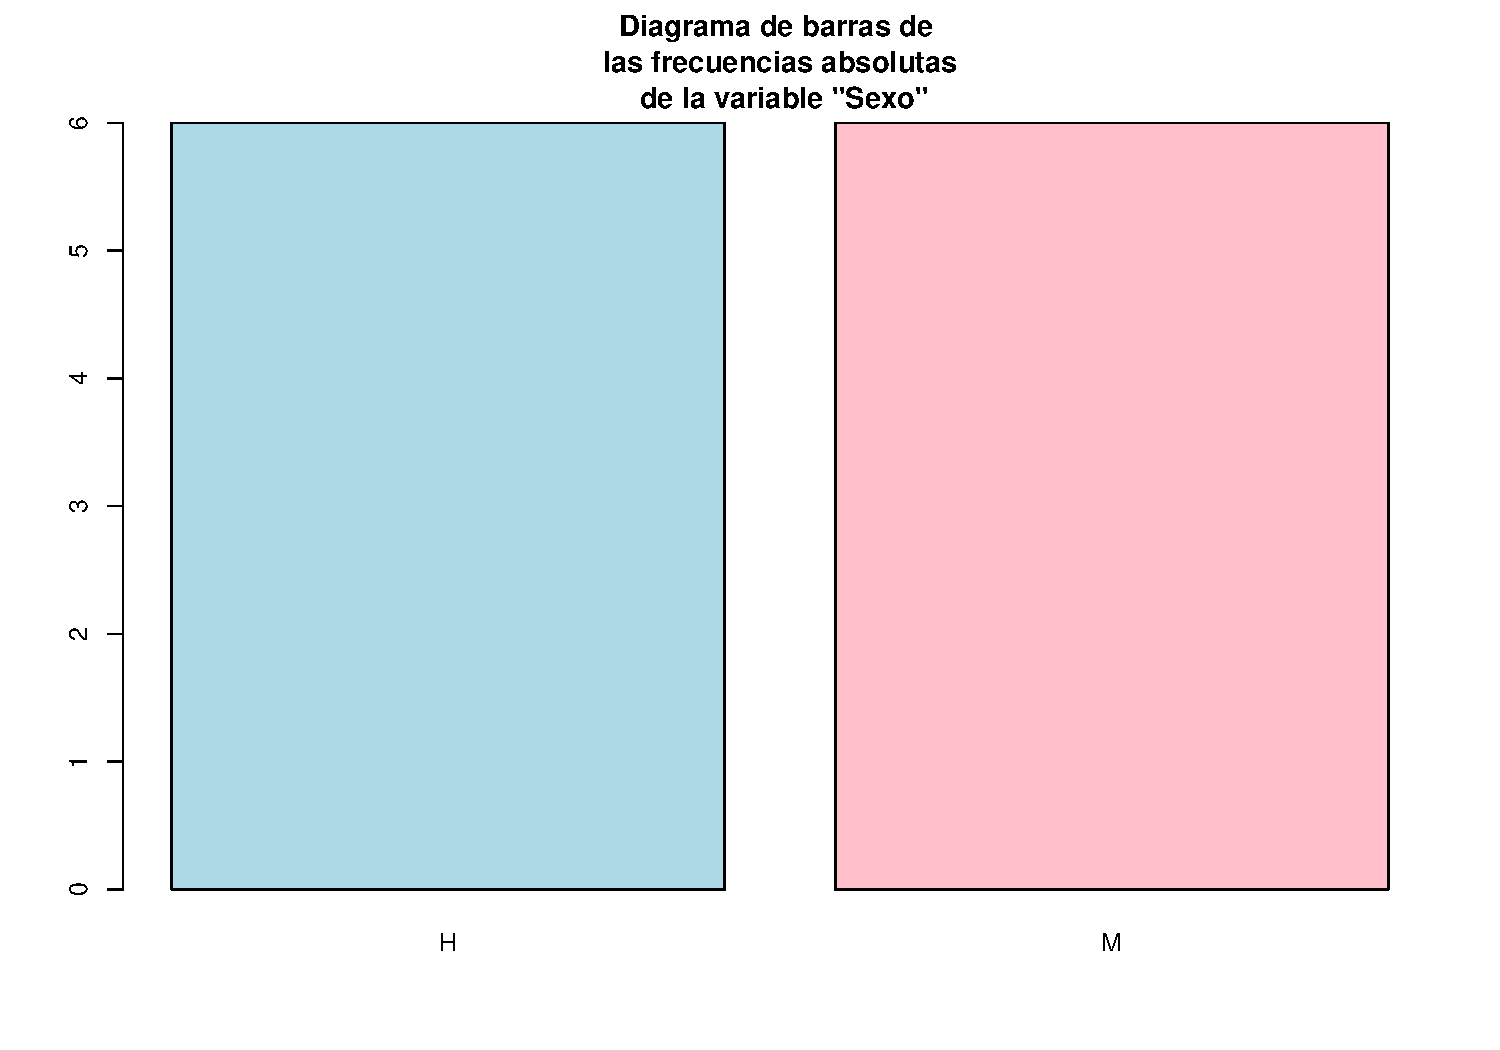
\includegraphics[width=250px]{Hora3_files/figure-beamer/unnamed-chunk-32-1} \end{center}
\end{frame}

\begin{frame}[fragile]{Diagrama de barras}
\protect\hypertarget{diagrama-de-barras-2}{}
\begin{Shaded}
\begin{Highlighting}[]
\FunctionTok{barplot}\NormalTok{(}\FunctionTok{prop.table}\NormalTok{(}\FunctionTok{table}\NormalTok{(Respuestas)), }
\AttributeTok{main=}\StringTok{"Diagrama de barras de frecuencias }
\StringTok{      relativas}\SpecialCharTok{\textbackslash{}n}\StringTok{ de la variable }\SpecialCharTok{\textbackslash{}"}\StringTok{Respuestas}\SpecialCharTok{\textbackslash{}"}\StringTok{"}\NormalTok{)}
\end{Highlighting}
\end{Shaded}

\begin{center}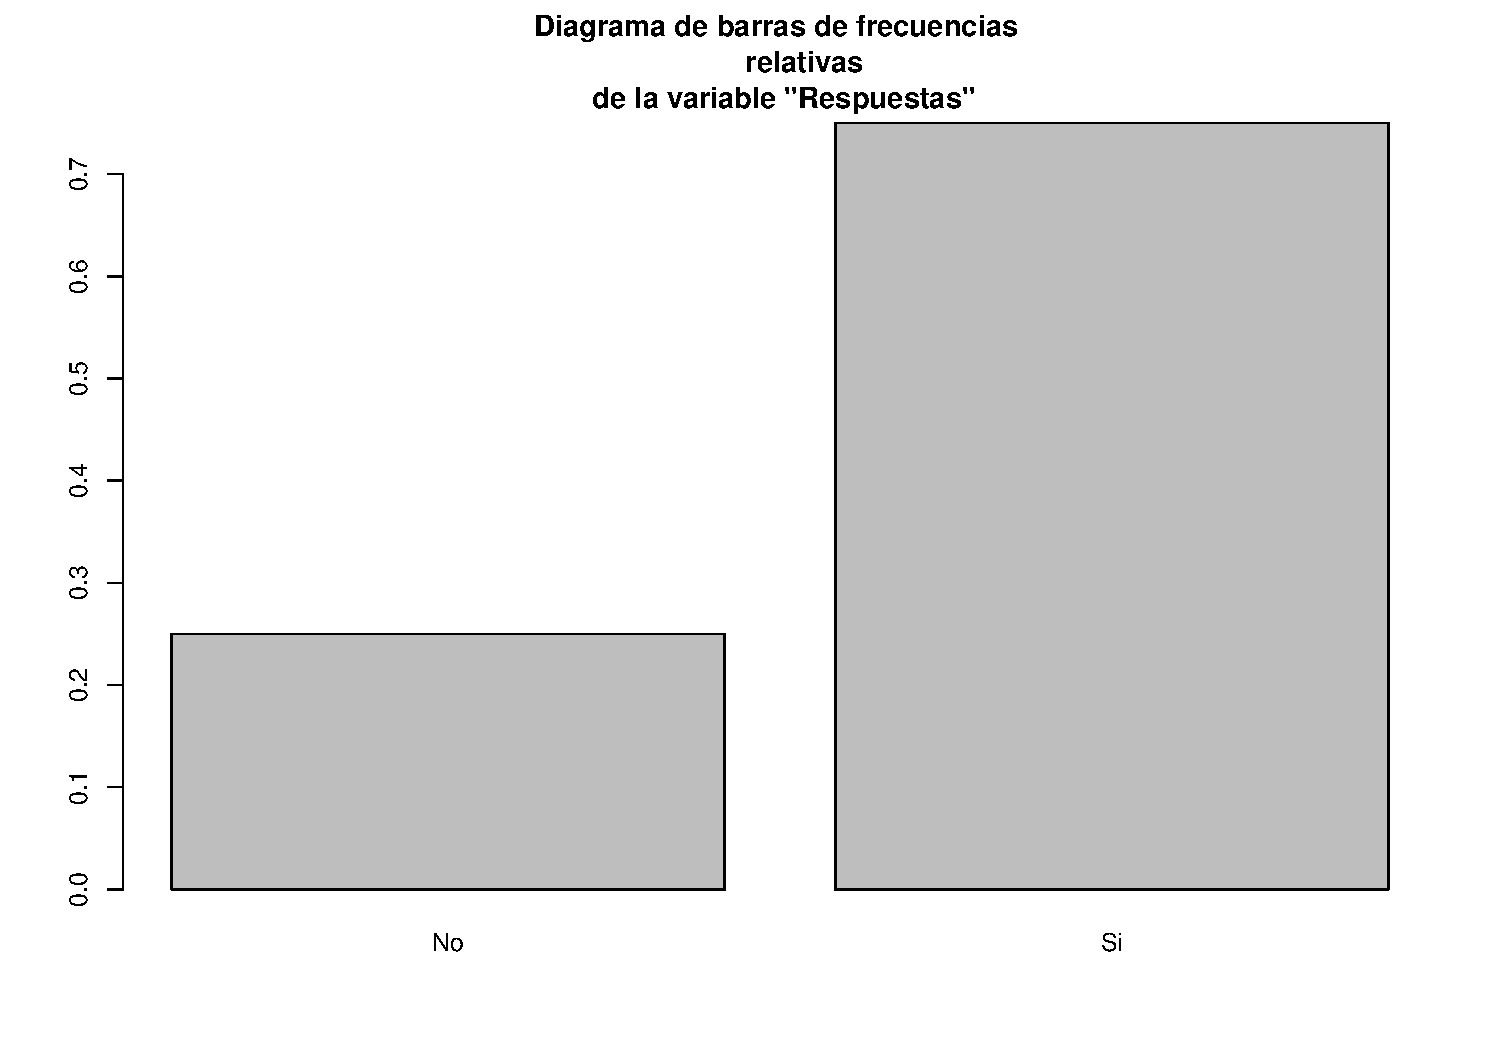
\includegraphics[width=250px]{Hora3_files/figure-beamer/unnamed-chunk-33-1} \end{center}
\end{frame}

\begin{frame}[fragile]{Diagrama de barras - Parámetros}
\protect\hypertarget{diagrama-de-barras---paruxe1metros}{}
Habréis observado que en las funciones \texttt{barplot()} anteriores
hemos usado el parámetro \texttt{main} para poner título a los
diagramas; en general, la función \texttt{barplot()} admite los
parámetros de \texttt{plot} que tienen sentido en el contexto de los
diagramas de barras: \texttt{xlab}, \texttt{ylab}, \texttt{main}, etc.
Los parámetros disponibles se pueden consultar en
\texttt{help(barplot)}. Aquí sólo vamos a comentar algunos.
\end{frame}

\begin{frame}[fragile]{Diagrama de barras - Colores}
\protect\hypertarget{diagrama-de-barras---colores}{}
\begin{Shaded}
\begin{Highlighting}[]
\FunctionTok{par}\NormalTok{(}\AttributeTok{mfrow=}\FunctionTok{c}\NormalTok{(}\DecValTok{1}\NormalTok{,}\DecValTok{2}\NormalTok{))}
\FunctionTok{barplot}\NormalTok{(}\FunctionTok{table}\NormalTok{(Respuestas), }\AttributeTok{col=}\FunctionTok{c}\NormalTok{(}\StringTok{"green"}\NormalTok{))}
\FunctionTok{barplot}\NormalTok{(}\FunctionTok{table}\NormalTok{(Respuestas), }\AttributeTok{col=}\FunctionTok{c}\NormalTok{(}\StringTok{"red"}\NormalTok{,}\StringTok{"blue"}\NormalTok{))}
\end{Highlighting}
\end{Shaded}

\begin{center}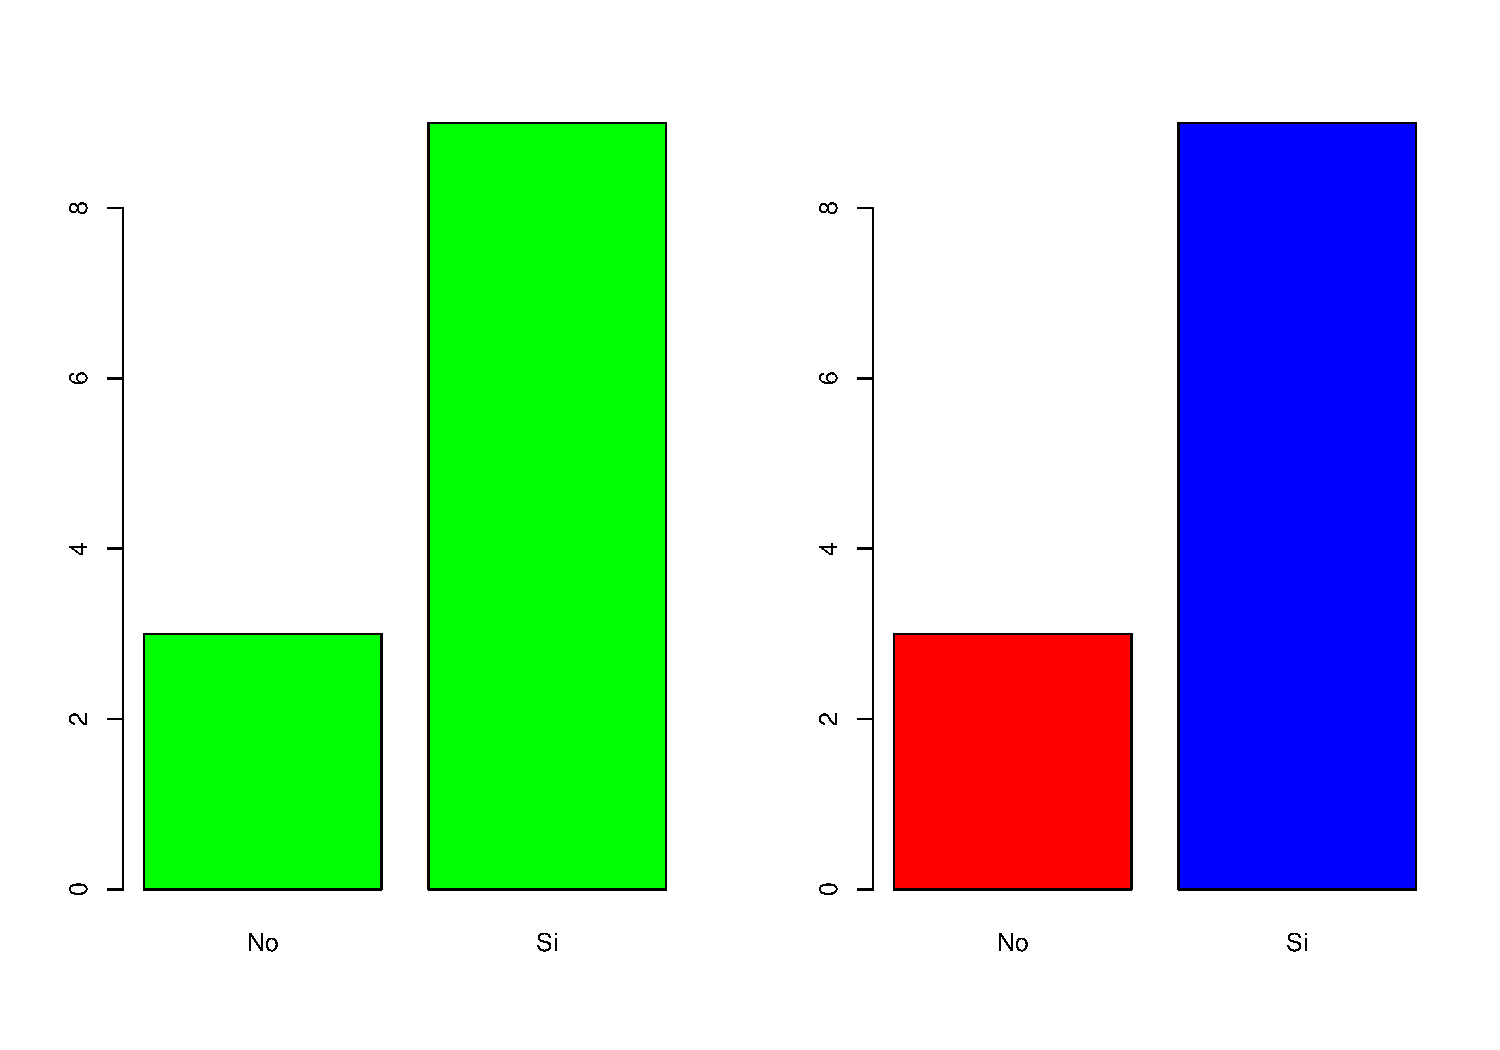
\includegraphics[width=250px]{Hora3_files/figure-beamer/unnamed-chunk-34-1} \end{center}

\begin{Shaded}
\begin{Highlighting}[]
\FunctionTok{par}\NormalTok{(}\AttributeTok{mfrow=}\FunctionTok{c}\NormalTok{(}\DecValTok{1}\NormalTok{,}\DecValTok{1}\NormalTok{))}
\end{Highlighting}
\end{Shaded}
\end{frame}

\begin{frame}[fragile]{Diagrama de barras - Colores}
\protect\hypertarget{diagrama-de-barras---colores-1}{}
\begin{Shaded}
\begin{Highlighting}[]
\FunctionTok{barplot}\NormalTok{(}\FunctionTok{table}\NormalTok{(x), }\AttributeTok{horiz=}\ConstantTok{TRUE}\NormalTok{)}
\end{Highlighting}
\end{Shaded}

\begin{center}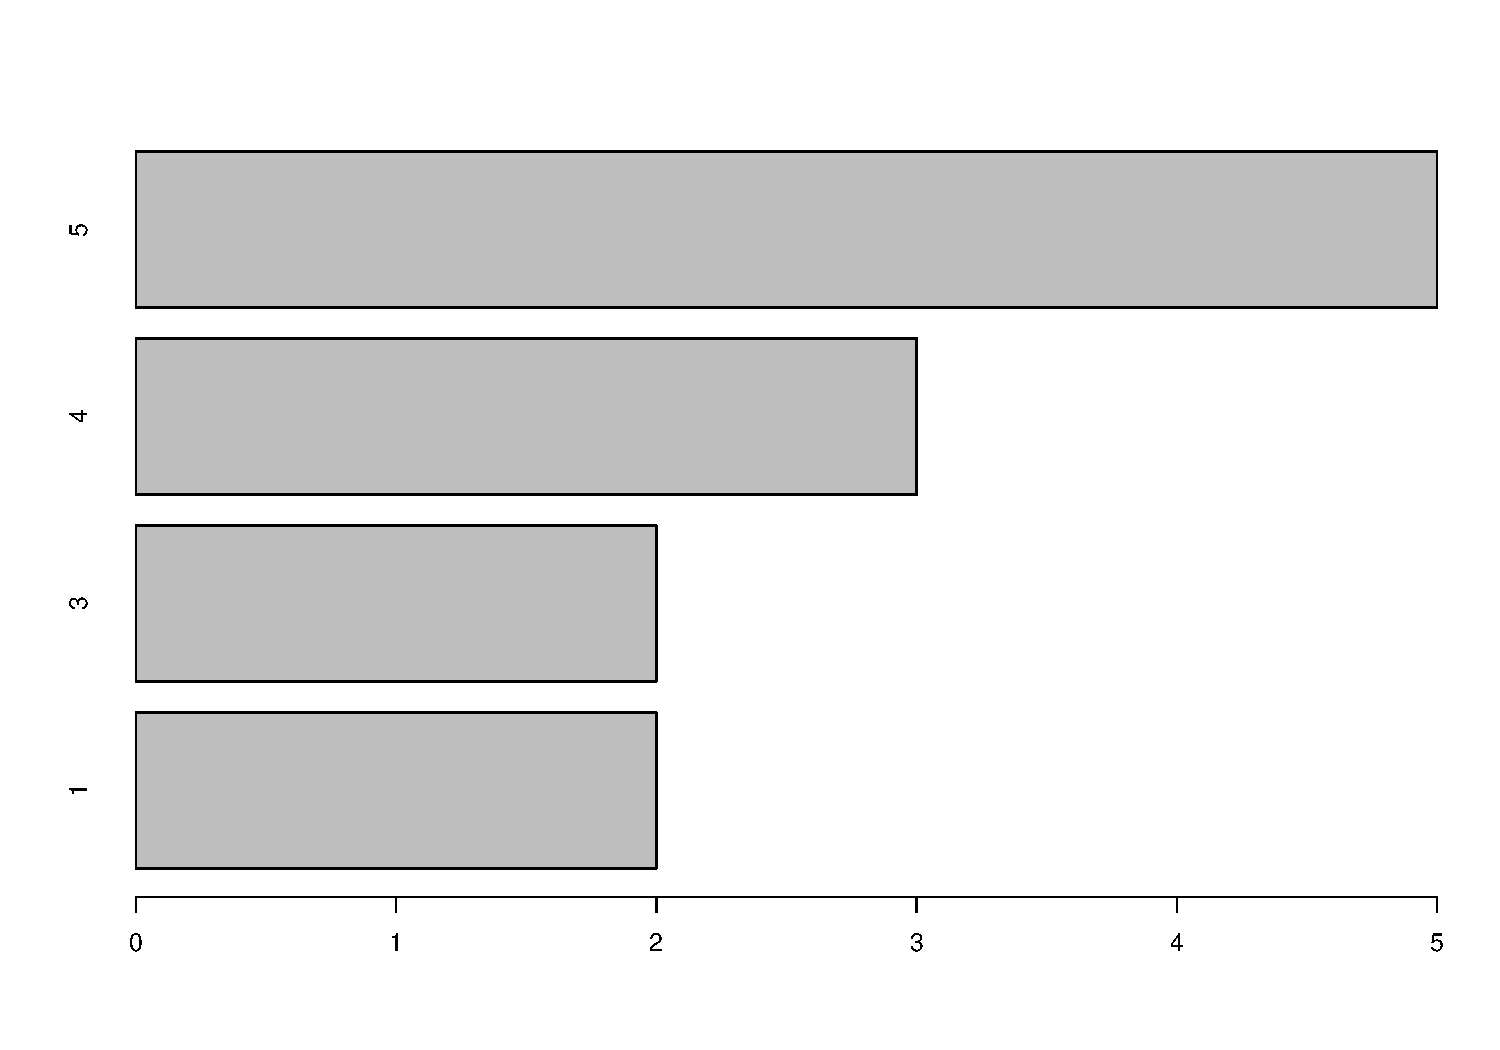
\includegraphics[width=275px]{Hora3_files/figure-beamer/unnamed-chunk-35-1} \end{center}
\end{frame}

\begin{frame}[fragile]{Diagrama de barras - Tabla bidimensional}
\protect\hypertarget{diagrama-de-barras---tabla-bidimensional}{}
\begin{Shaded}
\begin{Highlighting}[]
\FunctionTok{barplot}\NormalTok{(}\FunctionTok{table}\NormalTok{(Sexo,Respuestas), }\AttributeTok{legend.text =} \ConstantTok{TRUE}\NormalTok{)}
\end{Highlighting}
\end{Shaded}

\begin{center}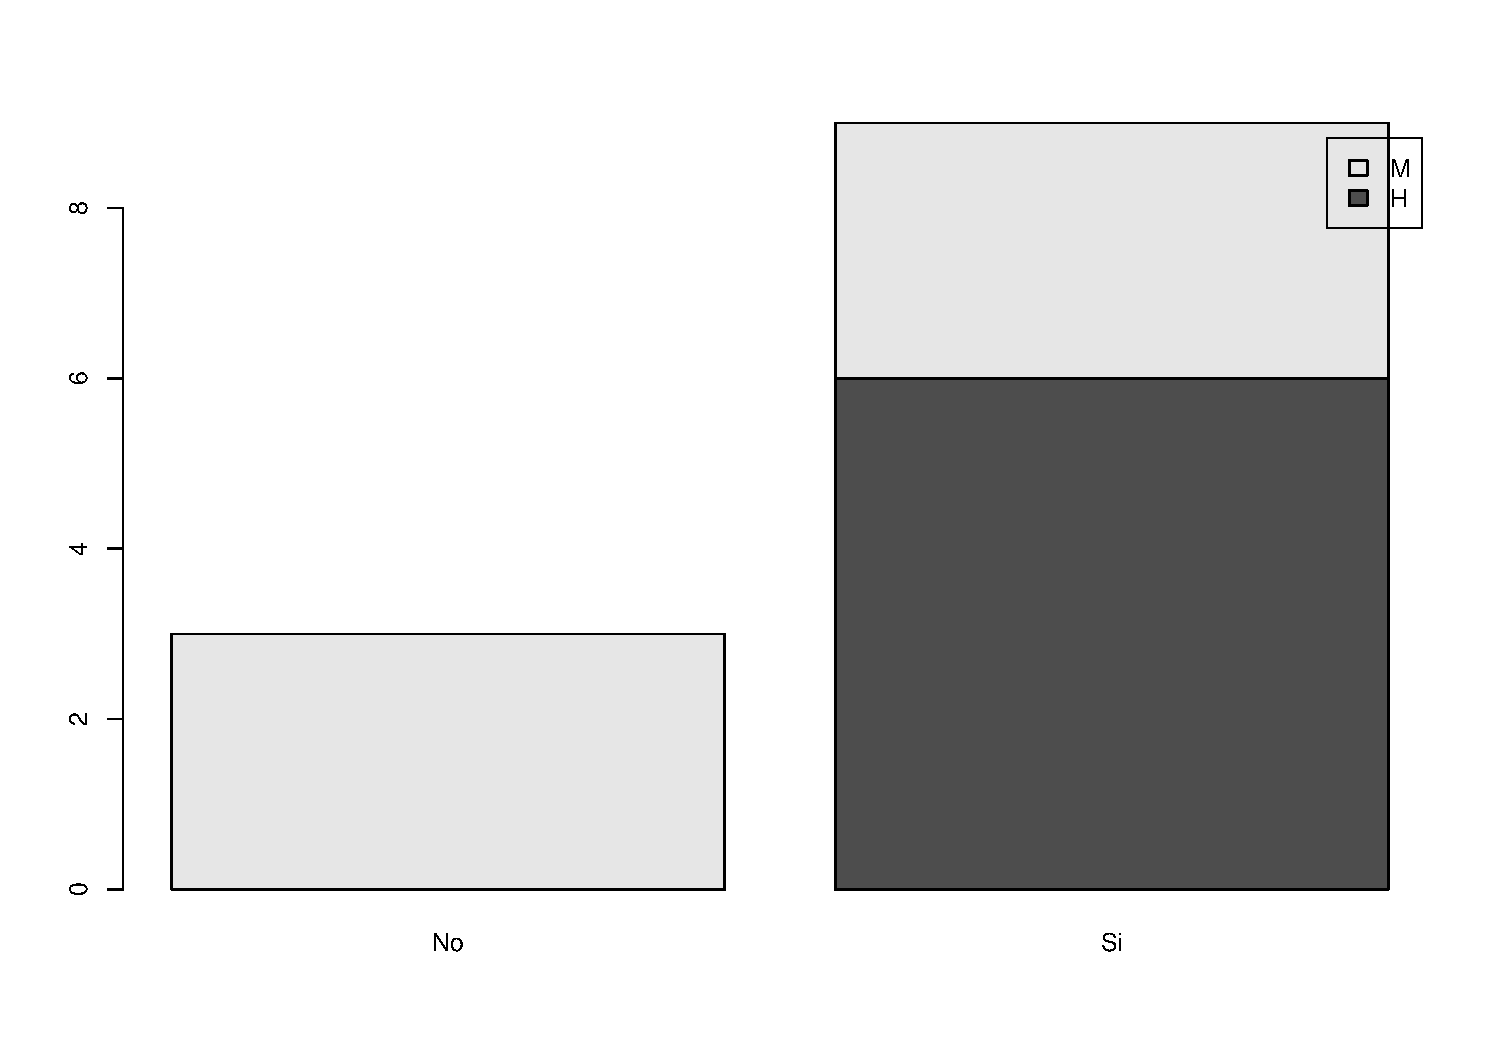
\includegraphics[width=275px]{Hora3_files/figure-beamer/unnamed-chunk-36-1} \end{center}
\end{frame}

\begin{frame}[fragile]{Diagrama de barras - Tabla bidimensional}
\protect\hypertarget{diagrama-de-barras---tabla-bidimensional-1}{}
\begin{Shaded}
\begin{Highlighting}[]
\FunctionTok{barplot}\NormalTok{(}\FunctionTok{table}\NormalTok{(Sexo,Respuestas), }\AttributeTok{beside=}\ConstantTok{TRUE}\NormalTok{, }
        \AttributeTok{legend.text=}\ConstantTok{TRUE}\NormalTok{)}
\end{Highlighting}
\end{Shaded}

\begin{center}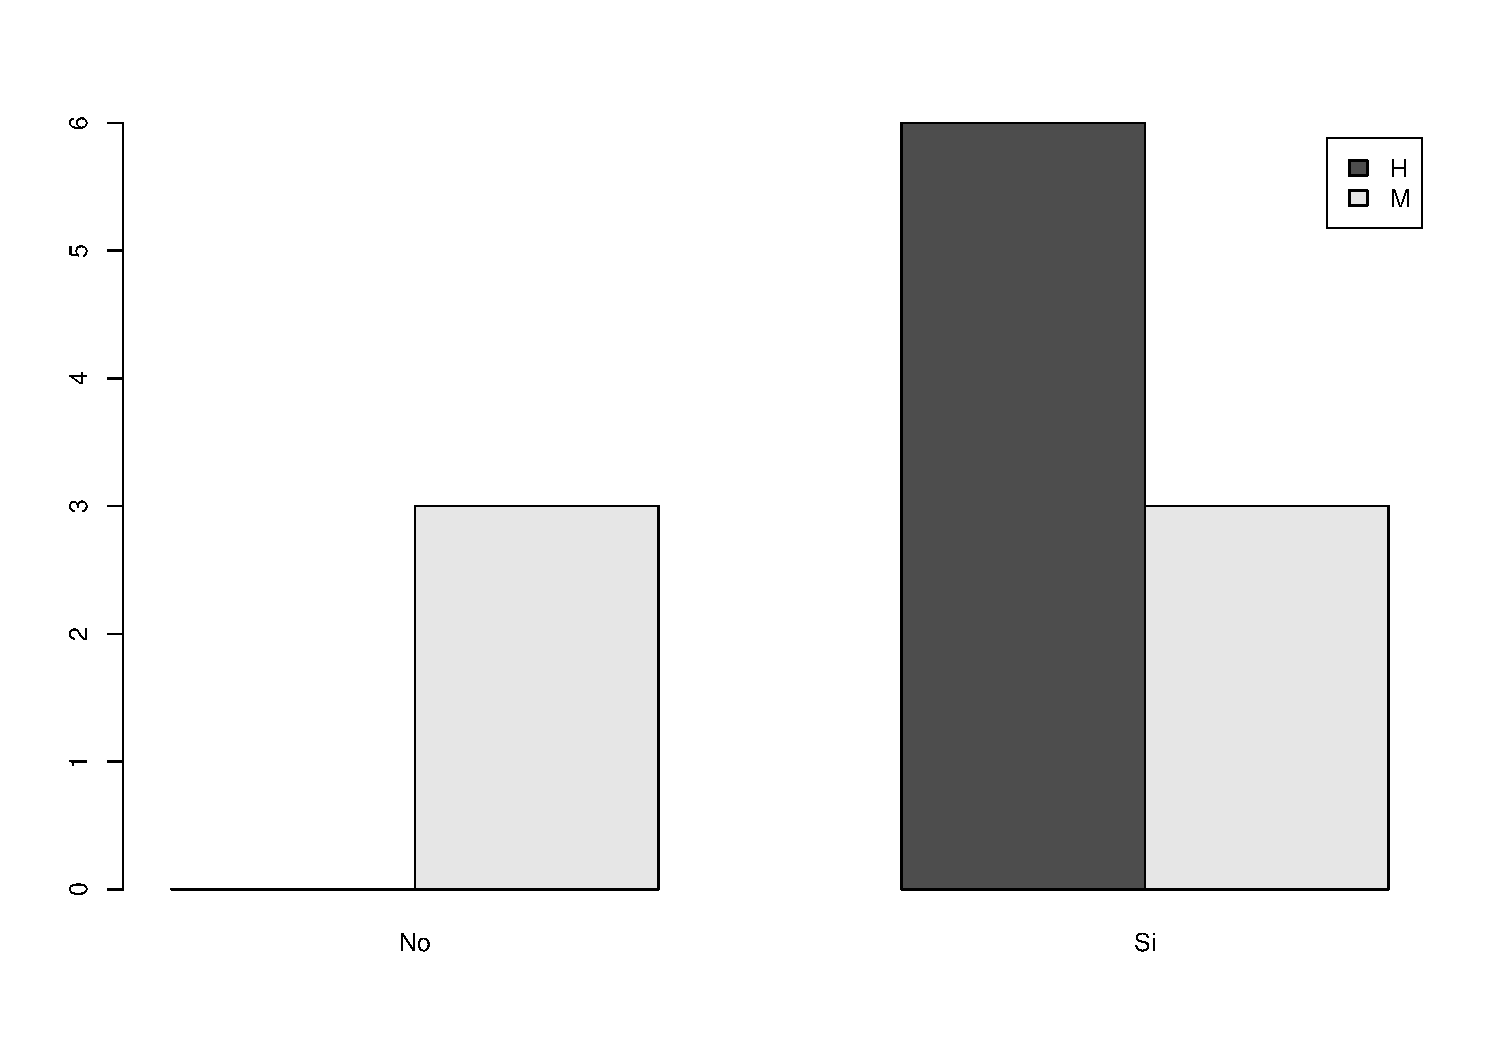
\includegraphics[width=270px]{Hora3_files/figure-beamer/unnamed-chunk-37-1} \end{center}
\end{frame}

\begin{frame}[fragile]{Diagrama de barras - Parámetros de las leyendas}
\protect\hypertarget{diagrama-de-barras---paruxe1metros-de-las-leyendas}{}
\begin{Shaded}
\begin{Highlighting}[]
\FunctionTok{barplot}\NormalTok{(}\FunctionTok{table}\NormalTok{(Respuestas,Sexo), }\AttributeTok{beside=}\ConstantTok{TRUE}\NormalTok{, }
        \AttributeTok{names=}\FunctionTok{c}\NormalTok{(}\StringTok{"Men"}\NormalTok{, }\StringTok{"Women"}\NormalTok{), }\AttributeTok{col=}\FunctionTok{c}\NormalTok{(}\StringTok{"yellow"}\NormalTok{,}\StringTok{"lightblue"}\NormalTok{),  }
        \AttributeTok{legend.text=}\FunctionTok{c}\NormalTok{(}\StringTok{"No"}\NormalTok{,}\StringTok{"Yes"}\NormalTok{))}
\end{Highlighting}
\end{Shaded}

\begin{center}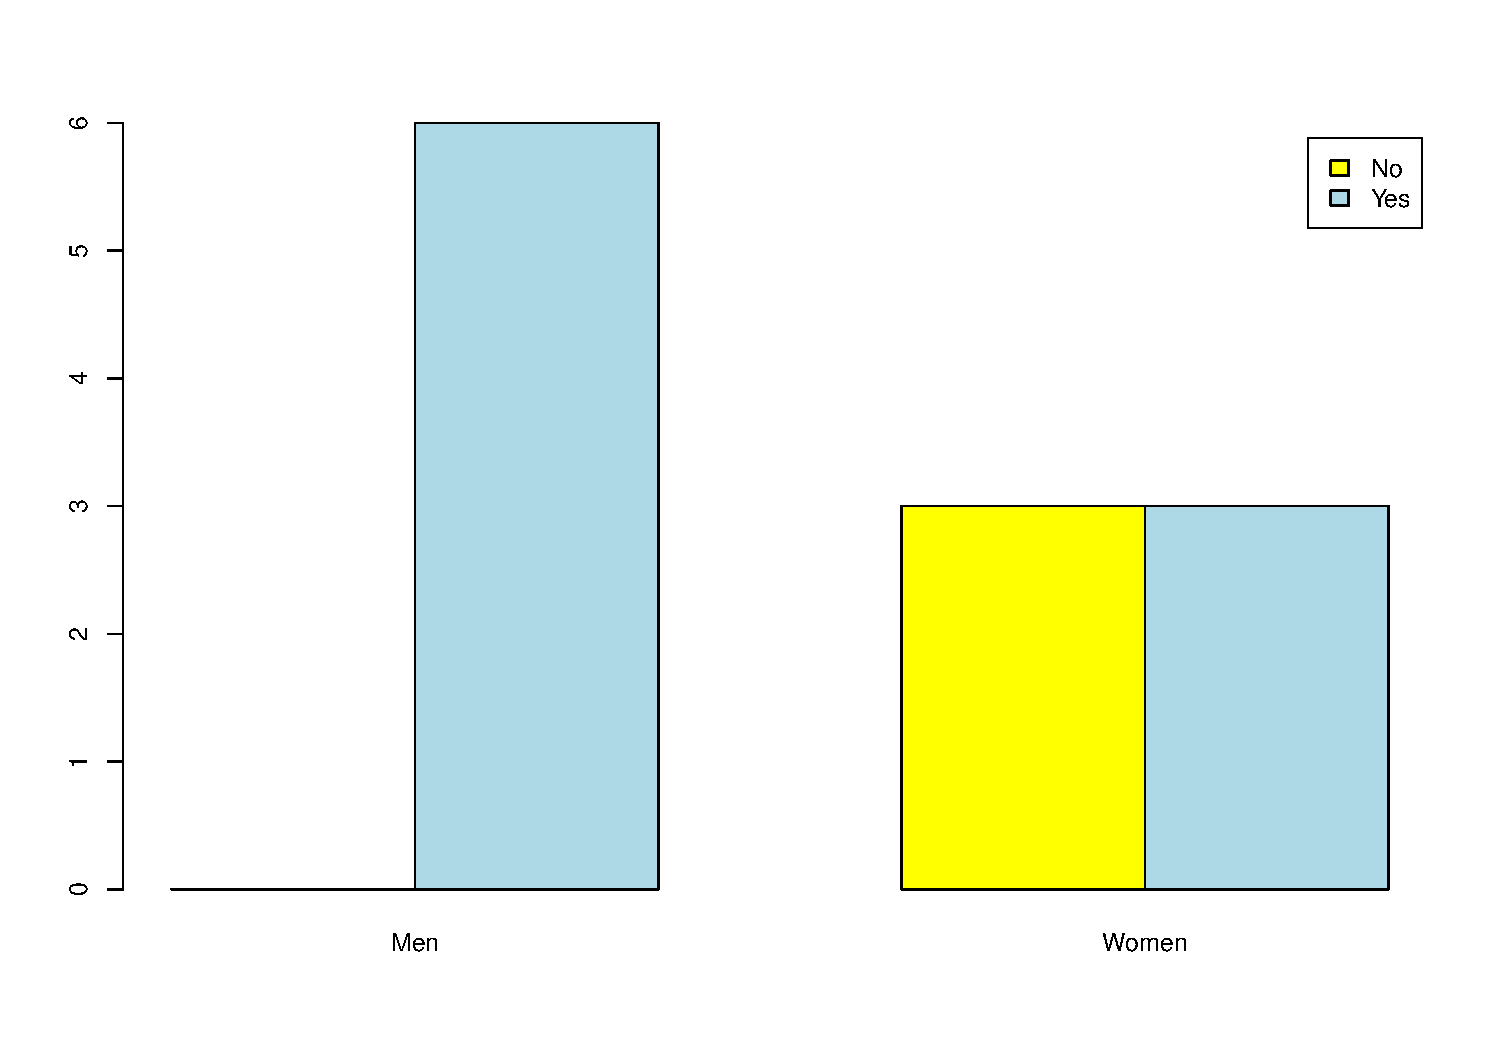
\includegraphics[width=250px]{Hora3_files/figure-beamer/unnamed-chunk-38-1} \end{center}
\end{frame}

\begin{frame}[fragile]{Diagrama circular}
\protect\hypertarget{diagrama-circular}{}
Un tipo muy popular de representación gráfica de variables cualitativas
son los \blue{diagramas circulares}. En un diagrama circular
(\texttt{pie\ chart}) se representan los niveles de una variable
cualitativa como sectores circulares de un círculo, de manera que el
ángulo (o equivalentemente, el área) de cada sector sea proporcional a
la frecuencia del nivel al que corresponde.

Con R, este tipo de diagramas se producen con la instrucción
\texttt{pie}, de nuevo aplicada a una tabla de frecuencias y no al
vector original.
\end{frame}

\begin{frame}[fragile]{Diagrama circular - Parámetros}
\protect\hypertarget{diagrama-circular---paruxe1metros}{}
La función \texttt{pie} admite muchos parámetros para modificar el
resultado: se pueden cambiar los colores con \texttt{col}, se pueden
cambiar los nombres de los niveles con \texttt{names}, se puede poner un
título con \texttt{main}, etc.; podéis consultar la lista completa de
parámetros en \texttt{help(pie)}.
\end{frame}

\begin{frame}[fragile]{Diagrama circular}
\protect\hypertarget{diagrama-circular-1}{}
\begin{Shaded}
\begin{Highlighting}[]
\NormalTok{x}
\end{Highlighting}
\end{Shaded}

\begin{verbatim}
##  [1] 1 3 5 5 4 3 4 5 5 1 5 4
\end{verbatim}

\begin{Shaded}
\begin{Highlighting}[]
\FunctionTok{pie}\NormalTok{(}\FunctionTok{table}\NormalTok{(x), }\AttributeTok{main=}\StringTok{"Diagrama circular de la variable x"}\NormalTok{)}
\end{Highlighting}
\end{Shaded}

\begin{center}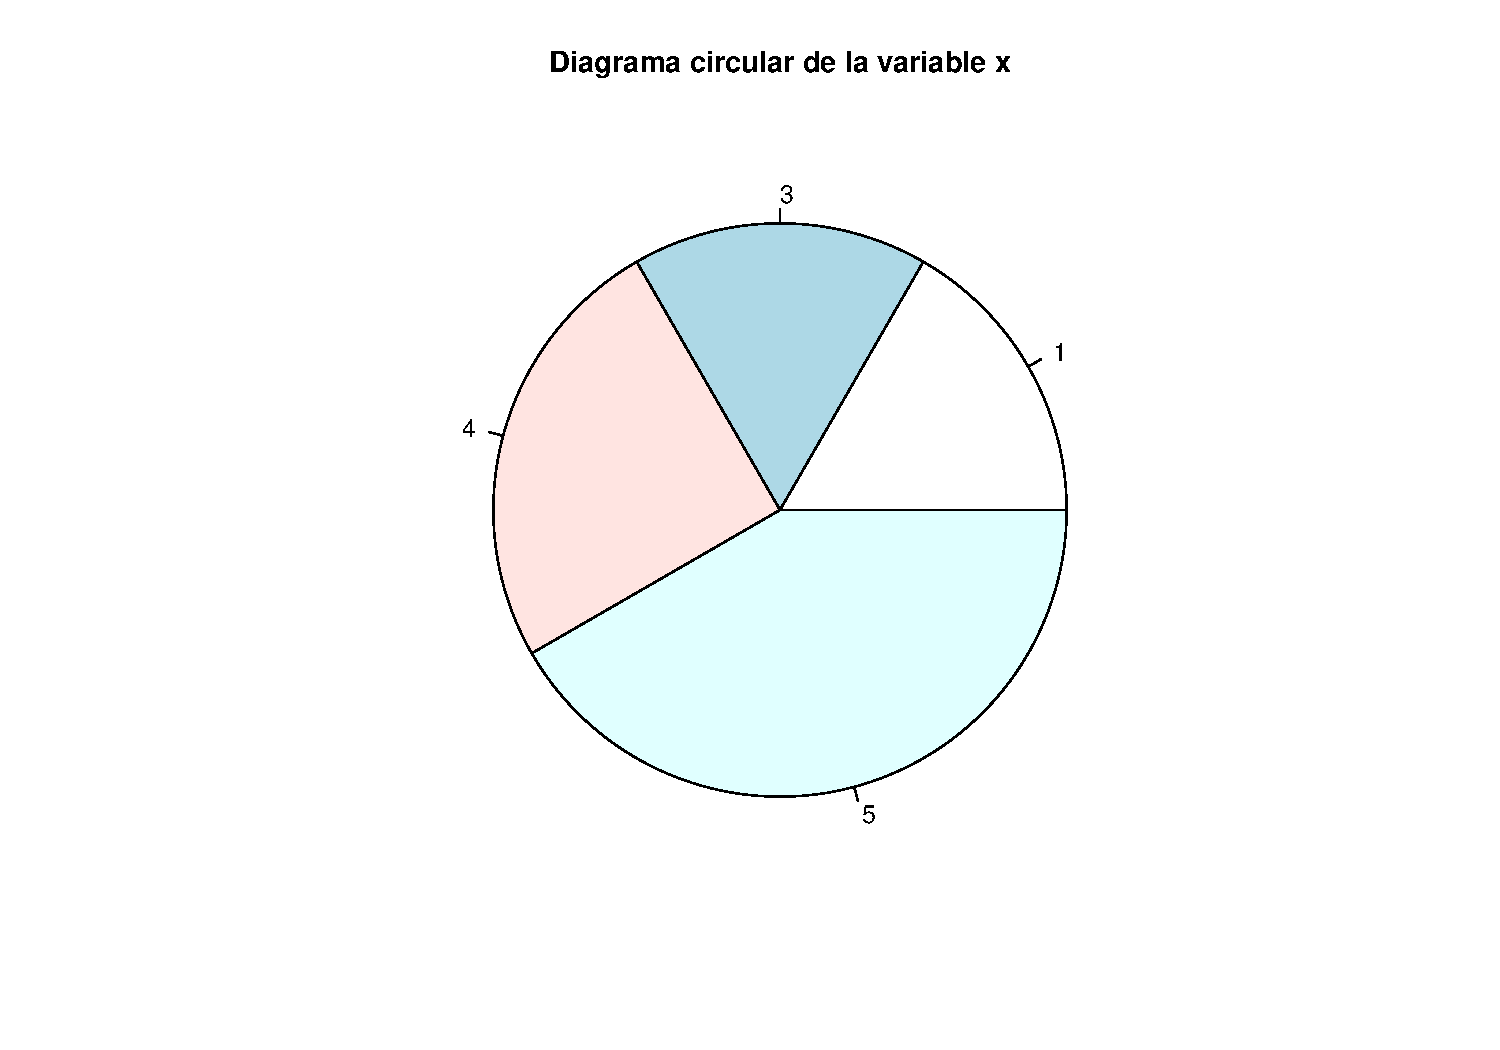
\includegraphics[width=275px]{Hora3_files/figure-beamer/unnamed-chunk-39-1} \end{center}
\end{frame}

\begin{frame}[fragile]{Diagrama circular}
\protect\hypertarget{diagrama-circular-2}{}
\begin{Shaded}
\begin{Highlighting}[]
\NormalTok{Respuestas}
\end{Highlighting}
\end{Shaded}

\begin{verbatim}
##  [1] No Si No Si Si Si Si Si Si Si No Si
## Levels: No Si
\end{verbatim}

\begin{Shaded}
\begin{Highlighting}[]
\FunctionTok{pie}\NormalTok{(}\FunctionTok{table}\NormalTok{(Respuestas), }\AttributeTok{main=}\StringTok{"Diagrama circular de la variable Respuestas"}\NormalTok{)}
\end{Highlighting}
\end{Shaded}

\begin{center}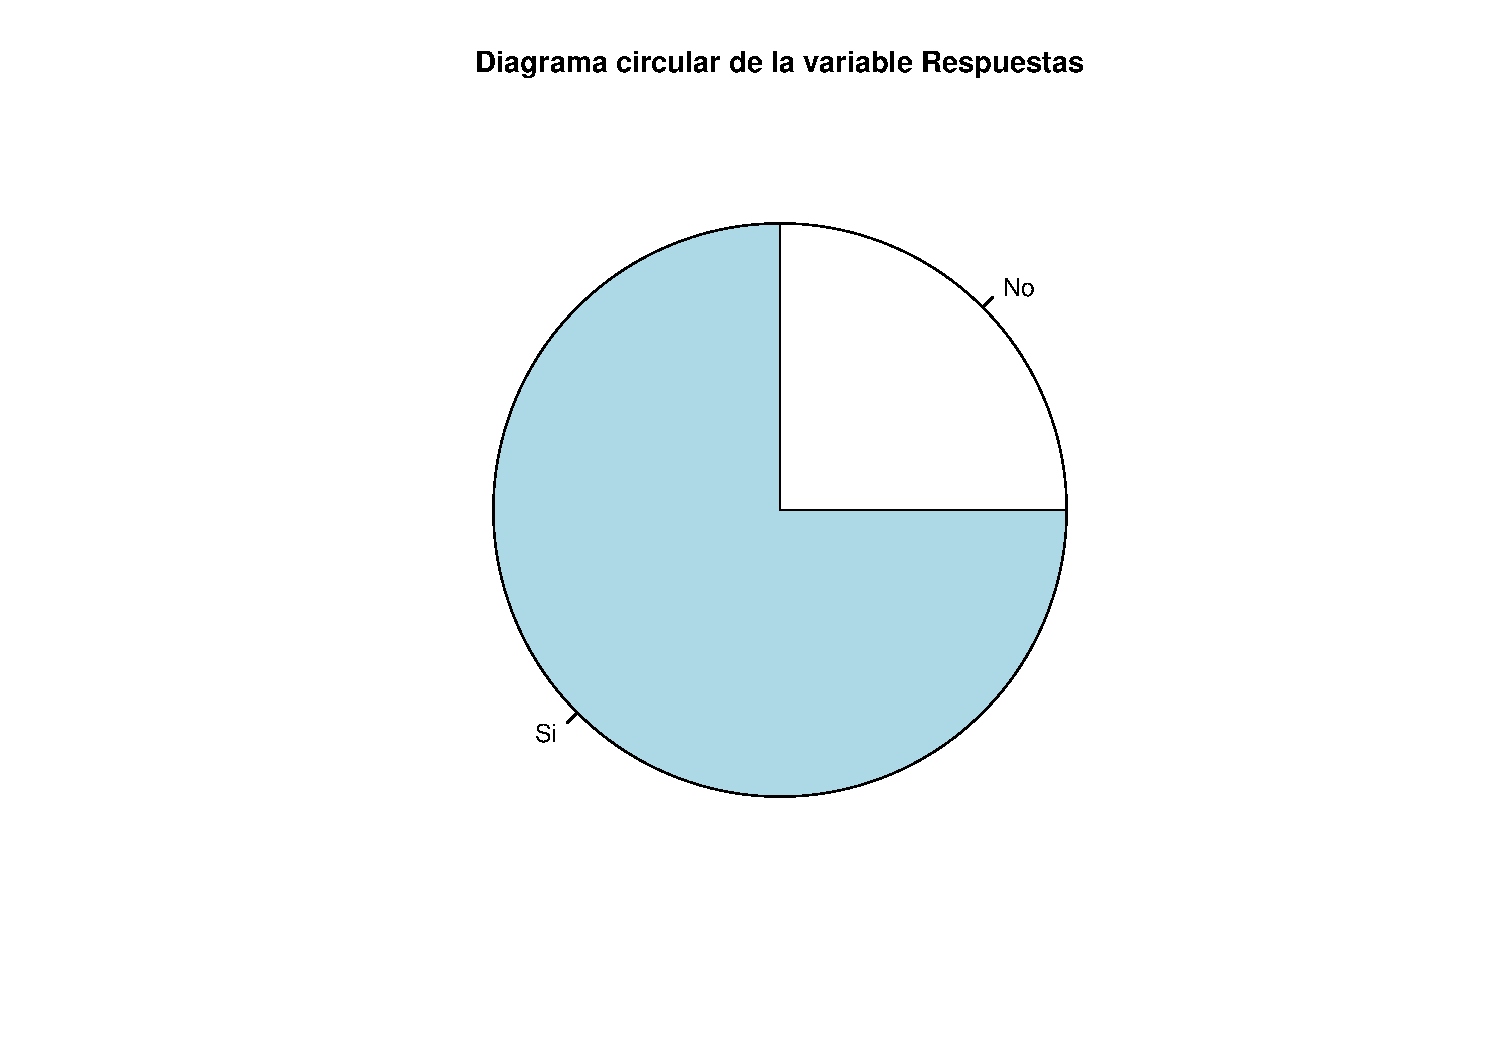
\includegraphics[width=250px]{Hora3_files/figure-beamer/unnamed-chunk-40-1} \end{center}
\end{frame}

\begin{frame}{Diagrama circular}
\protect\hypertarget{diagrama-circular-3}{}
Pese a su popularidad, es poco recomendable usar diagramas circulares
porque a veces es difícil, a simple vista, comprender las relaciones
entre las frecuencias que representan.
\end{frame}

\begin{frame}[fragile]{Gráficos de mosaico}
\protect\hypertarget{gruxe1ficos-de-mosaico}{}
Otra representación de las tablas multidimensionales de frecuencias son
los \blue{gráficos de mosaico}. Estos gráficos se obtienen sustituyendo
cada entrada de la tabla de frecuencias por una región rectangular de
área proporcional a su valor.

En concreto, para obtener el gráfico de mosaico de una tabla
bidimensional, se parte de un cuadrado de lado 1, primero se divide en
barras verticales de amplitudes iguales a las frecuencias relativas de
una variable, y luego cada barra se divide, a lo alto, en regiones de
alturas proporcionales a las frecuencias relativas marginales de cada
nivel de la otra variable, dentro del nivel correspondiente de la
primera variable.

Un gráfico de mosaico de una tabla se obtiene con R aplicando la función
\texttt{plot} a la tabla, o también la función \texttt{mosaicplot}. Esta
última también se puede aplicar a matrices.
\end{frame}

\begin{frame}[fragile]{Gráficos de mosaico}
\protect\hypertarget{gruxe1ficos-de-mosaico-1}{}
\begin{Shaded}
\begin{Highlighting}[]
\FunctionTok{plot}\NormalTok{(}\FunctionTok{table}\NormalTok{(Sexo,Respuestas), }
\AttributeTok{main=}\StringTok{"Gráfico de mosaico de las variables}
\StringTok{  }\SpecialCharTok{\textbackslash{}"}\StringTok{Sexo}\SpecialCharTok{\textbackslash{}"}\StringTok{ y }\SpecialCharTok{\textbackslash{}"}\StringTok{Respuestas}\SpecialCharTok{\textbackslash{}"}\StringTok{"}\NormalTok{)}
\end{Highlighting}
\end{Shaded}

\begin{center}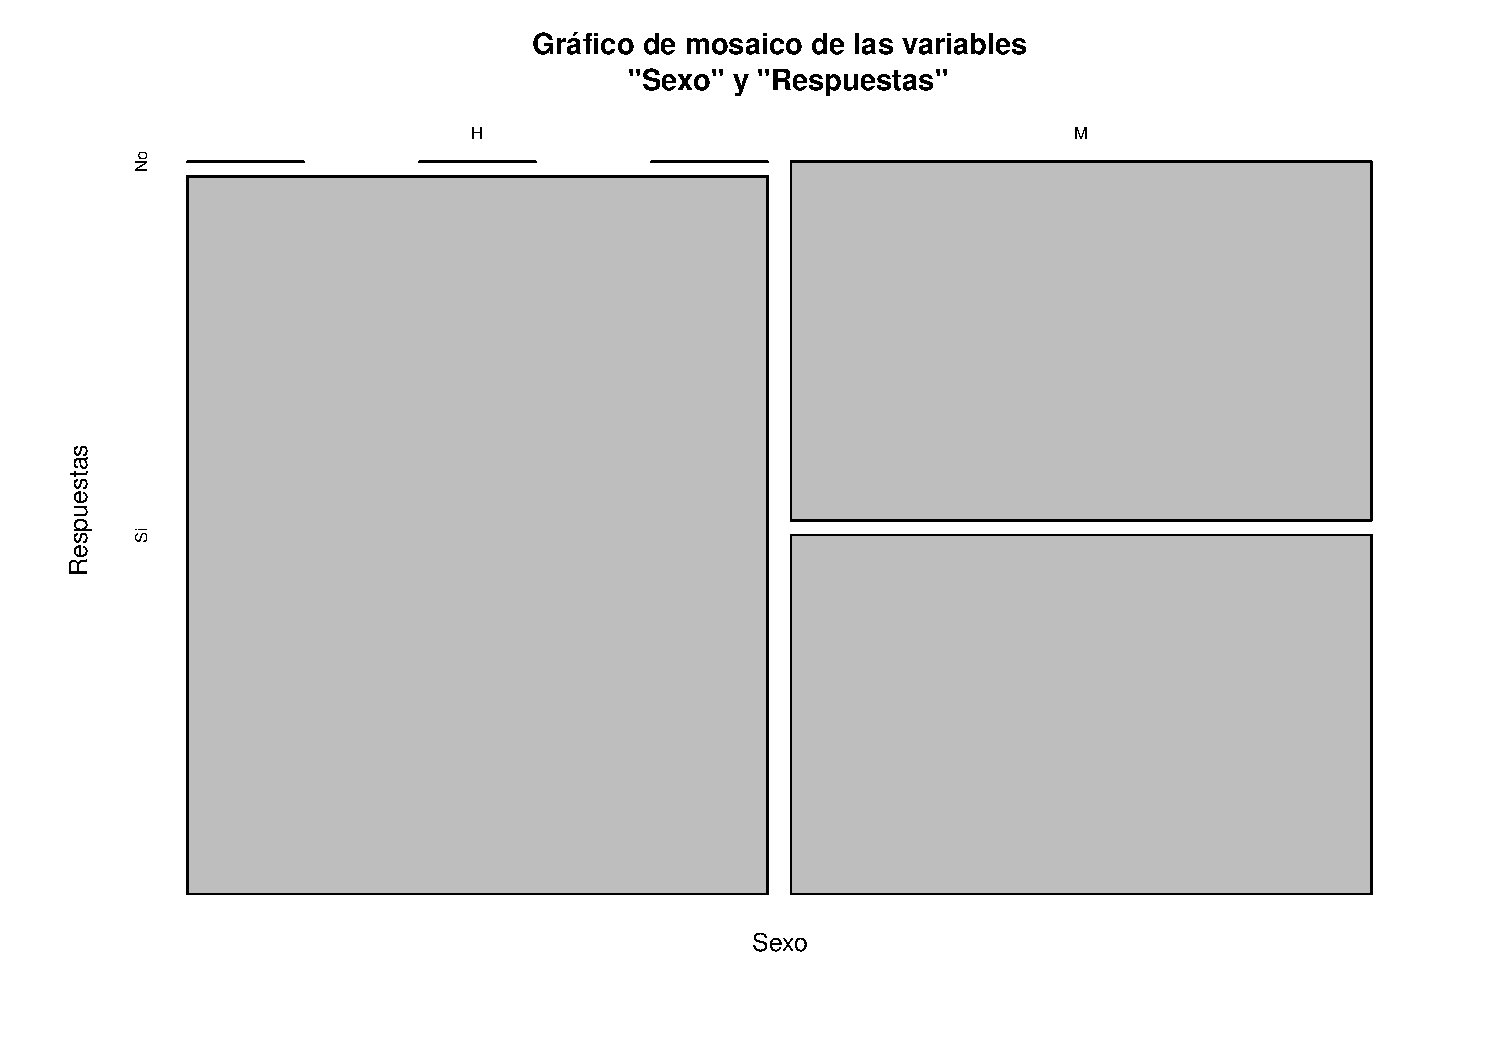
\includegraphics[width=250px]{Hora3_files/figure-beamer/unnamed-chunk-41-1} \end{center}
\end{frame}

\begin{frame}{Gráficos de mosaico}
\protect\hypertarget{gruxe1ficos-de-mosaico-2}{}
En el gráfico de mosaico de una tabla tridimensional, primero se divide
el cuadrado en barras verticales de amplitudes iguales a las frecuencias
relativas de una variable.

Luego cada barra se divide, a lo alto, en regiones de alturas
proporcionales a las frecuencias relativas marginales de cada nivel de
una segunda variable, dentro del nivel correspondiente de la primera
variable.

Finalmente, cada sector rectangular se vuelve a dividir a lo ancho en
regiones de amplitudes proporcionales a las frecuencias relativas
marginales de cada nivel de la tercera variable dentro de la combinación
correspondiente de niveles de las otras dos.
\end{frame}

\begin{frame}[fragile]{Gráficos de mosaico}
\protect\hypertarget{gruxe1ficos-de-mosaico-3}{}
\begin{Shaded}
\begin{Highlighting}[]
\FunctionTok{plot}\NormalTok{(HairEyeColor, }\AttributeTok{main=}\StringTok{"Gráfico de mosaico de la tabla HairEyeColor"}\NormalTok{, }
     \AttributeTok{col=}\FunctionTok{c}\NormalTok{(}\StringTok{"pink"}\NormalTok{,}\StringTok{"lightblue"}\NormalTok{))}
\end{Highlighting}
\end{Shaded}

\begin{center}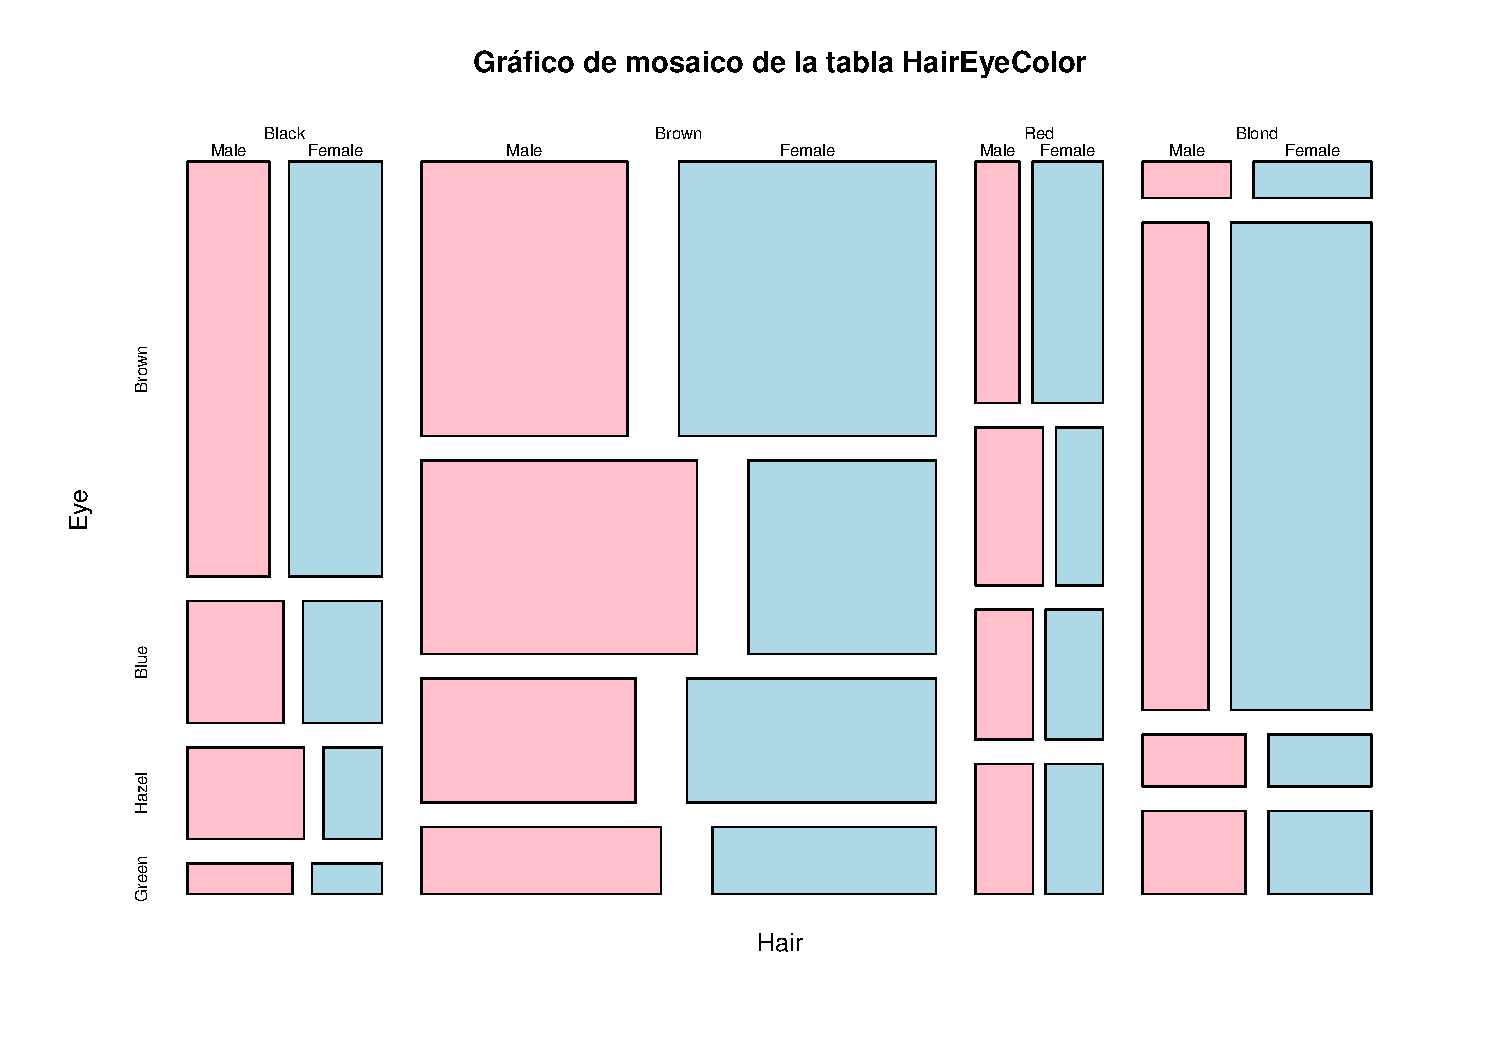
\includegraphics[width=270px]{Hora3_files/figure-beamer/unnamed-chunk-42-1} \end{center}
\end{frame}

\begin{frame}[fragile]{Muchos más gráficos}
\protect\hypertarget{muchos-muxe1s-gruxe1ficos}{}
Además de sus parámetros usuales, la función \texttt{plot} admite
algunos parámetros específicos cuando se usa para producir el gráfico de
mosaico de una tabla. Estos parámetros se pueden consultar en
\texttt{help(mosaicplot)}.

Los paquetes \texttt{vcd} y \texttt{vcdExtra} incluyen otras funciones
que producen representaciones gráficas interesantes de tablas
tridimensionales.

\begin{itemize}
\tightlist
\item
  La función \texttt{cotabplot} de \texttt{vcd} produce un diagrama de
  mosaico para cada nivel de la tercera variable.
\item
  La función \texttt{mosaic3d} de \texttt{vcdExtra} produce un diagrama
  de mosaico tridimensional en una ventana de una aplicación para
  gráficos 3D interactivos.
\end{itemize}
\end{frame}

\hypertarget{ejemplo-final}{%
\section{Ejemplo final}\label{ejemplo-final}}

\begin{frame}[fragile]{Un ejemplo final}
\protect\hypertarget{un-ejemplo-final}{}
Vamos a llevar a cabo un análisis completo de un ejemplo con lo que
hemos aprendido en esta lección y aprovecharemos para aprender algo
nuevo.

El objeto de datos \texttt{HairEyeColor} que lleva predefinido R es una
tabla de frecuencias absolutas de tres variables cualitativas: color de
cabello (\texttt{Hair}), color de los ojos (\texttt{Eye}) y sexo
(\texttt{Sex}).

Vamos a extraer de esta tabla una tabla bidimensional de frecuencias
absolutas de las variables \texttt{Eye} y \texttt{Hair}, sin distinguir
según el sexo. La manera más sencilla de obtener esta tabla es sumando
las subtablas de frecuencias para hombres y mujeres, y aplicando
\texttt{as.table()} al resultado para transformarlo en una
\texttt{table} por si no lo es.
\end{frame}

\begin{frame}[fragile]{Un ejemplo final}
\protect\hypertarget{un-ejemplo-final-1}{}
Vamos a traducir al castellano los nombres de las variables de esta
tabla y de sus niveles. Esto lo podemos llevar a cabo en un solo paso
con la función \texttt{dimnames()} que ya usamos sobre data frames. El
resultado de aplicar esta función a una table es una \texttt{list} cuyas
componentes son los niveles de cada variable.

\begin{Shaded}
\begin{Highlighting}[]
\FunctionTok{dimnames}\NormalTok{(HEC)}
\end{Highlighting}
\end{Shaded}

\begin{verbatim}
## $Hair
## [1] "Black" "Brown" "Red"   "Blond"
## 
## $Eye
## [1] "Brown" "Blue"  "Hazel" "Green"
\end{verbatim}

\textbf{Ejercicio.}

Redefinid dicha \texttt{list} para tener los niveles de los factores en
castellano
\end{frame}

\begin{frame}{Un ejemplo final}
\protect\hypertarget{un-ejemplo-final-2}{}
Vamos a dibujar un diagrama de mosaico de esta tabla, para visualizar
gráficamente sus entradas.

\begin{center}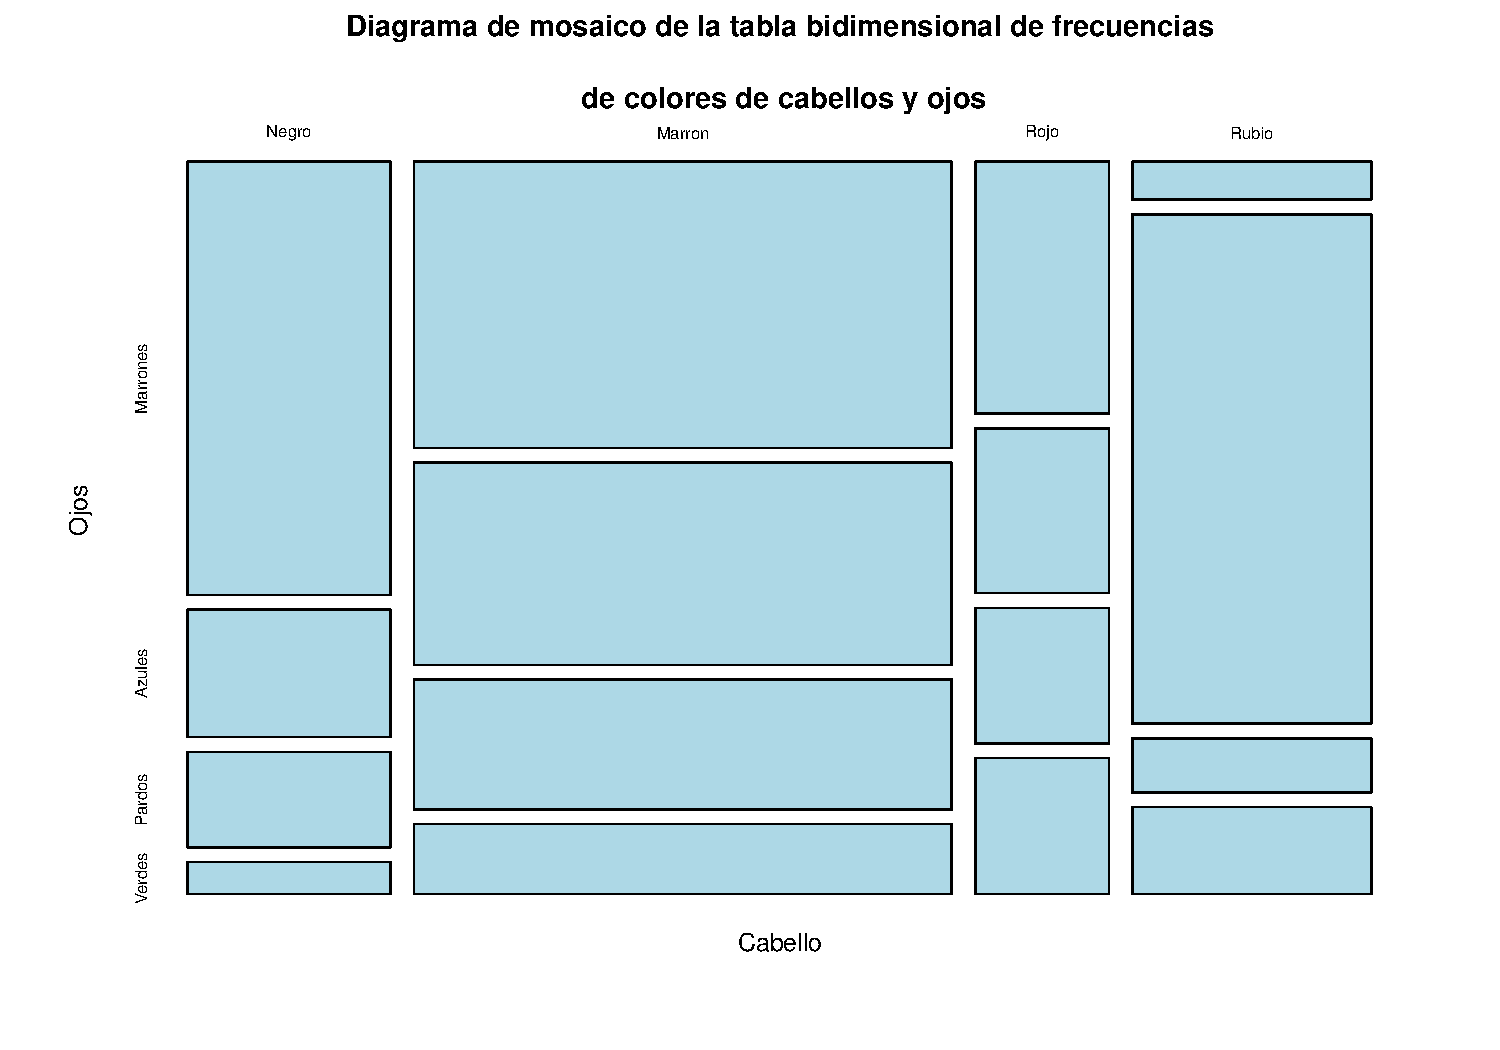
\includegraphics[width=275px]{Hora3_files/figure-beamer/unnamed-chunk-48-1} \end{center}
\end{frame}

\begin{frame}[fragile]{Un ejemplo final}
\protect\hypertarget{un-ejemplo-final-3}{}
A continuación, vamos a calcular el número total de individuos
representados en esta tabla:

\begin{verbatim}
## [1] 592
\end{verbatim}
\end{frame}

\begin{frame}[fragile]{Un ejemplo final}
\protect\hypertarget{un-ejemplo-final-4}{}
Las tablas de frecuencias absolutas y relativas de cada variable,

\begin{verbatim}
## Marrones   Azules   Pardos   Verdes 
##      220      215       93       64
\end{verbatim}

\begin{verbatim}
##  Negro Marron   Rojo  Rubio 
##    108    286     71    127
\end{verbatim}

\begin{verbatim}
## Marrones   Azules   Pardos   Verdes 
##    0.372    0.363    0.157    0.108
\end{verbatim}

\begin{verbatim}
##  Negro Marron   Rojo  Rubio 
##  0.182  0.483  0.120  0.215
\end{verbatim}
\end{frame}

\begin{frame}{Un ejemplo final}
\protect\hypertarget{un-ejemplo-final-5}{}
Representaremos estas últimas en sendos diagramas de barras.

\begin{center}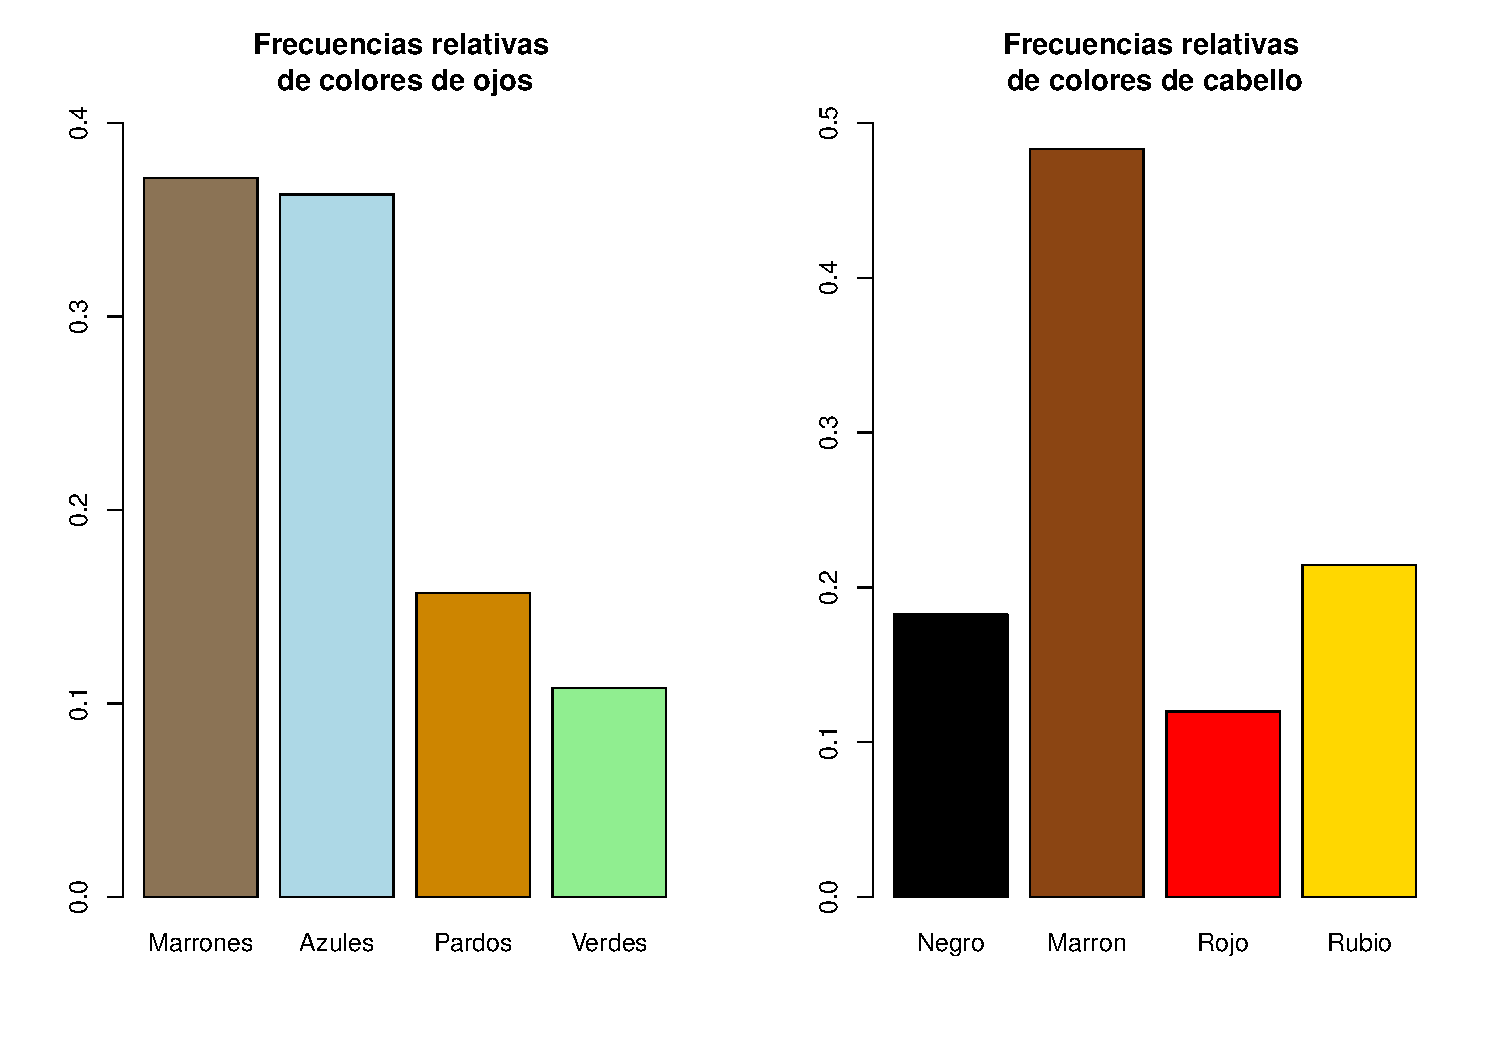
\includegraphics[width=275px]{Hora3_files/figure-beamer/unnamed-chunk-51-1} \end{center}
\end{frame}

\begin{frame}[fragile]{Un ejemplo final}
\protect\hypertarget{un-ejemplo-final-6}{}
En el diagrama anterior vemos que el color dominante de cabellos es el
castaño, mientras que en el color de ojos el marrón y el azul están
prácticamente empatados. Pasamos ahora a calcular las tablas de
frecuencias relativas y dibujar los dos diagramas de barras de las
frecuencias relativas marginales.

\begin{verbatim}
##         Ojos
## Cabello  Marrones Azules Pardos Verdes
##   Negro     0.115  0.034  0.025  0.008
##   Marron    0.201  0.142  0.091  0.049
##   Rojo      0.044  0.029  0.024  0.024
##   Rubio     0.012  0.159  0.017  0.027
\end{verbatim}
\end{frame}

\begin{frame}[fragile]{Un ejemplo final}
\protect\hypertarget{un-ejemplo-final-7}{}
\begin{verbatim}
##         Ojos
## Cabello  Marrones Azules Pardos Verdes
##   Negro     0.630  0.185  0.139  0.046
##   Marron    0.416  0.294  0.189  0.101
##   Rojo      0.366  0.239  0.197  0.197
##   Rubio     0.055  0.740  0.079  0.126
\end{verbatim}

\begin{verbatim}
##         Ojos
## Cabello  Marrones Azules Pardos Verdes
##   Negro     0.309  0.093  0.161  0.078
##   Marron    0.541  0.391  0.581  0.453
##   Rojo      0.118  0.079  0.151  0.219
##   Rubio     0.032  0.437  0.108  0.250
\end{verbatim}
\end{frame}

\begin{frame}{Un ejemplo final}
\protect\hypertarget{un-ejemplo-final-8}{}
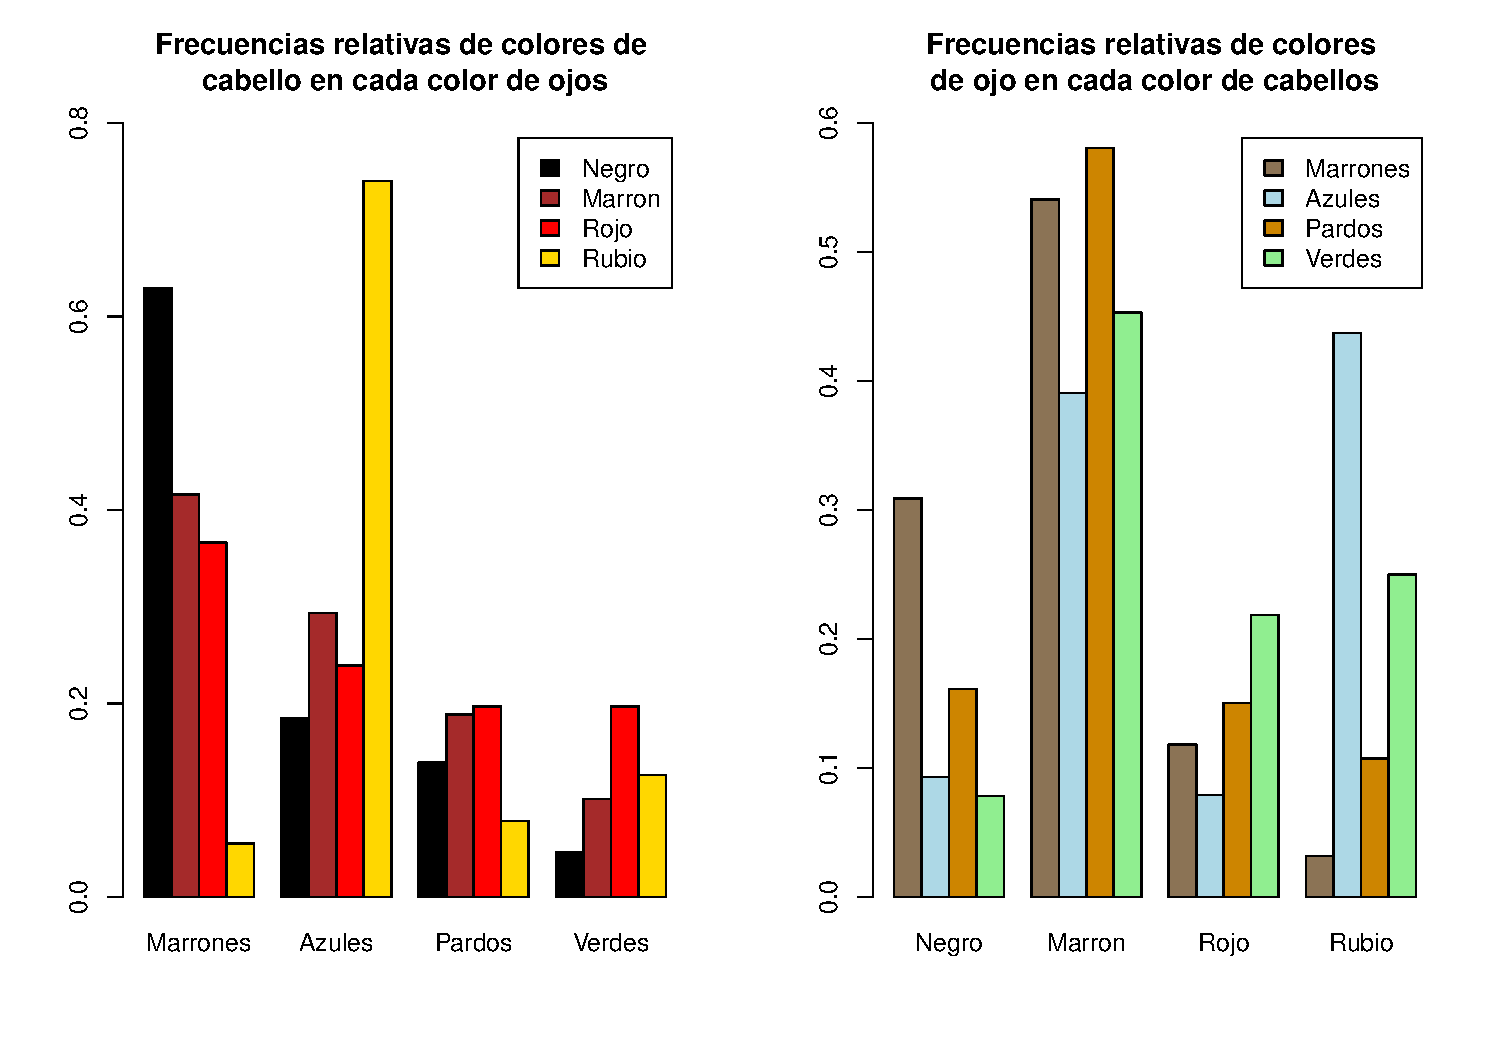
\includegraphics{Hora3_files/figure-beamer/unnamed-chunk-54-1.pdf}

Vemos que entre las personas de ojos azules, los cabellos rubios son los
más frecuentes, y que entre las personas castañas el color de ojos más
frecuente es el pardo.
\end{frame}

\begin{frame}[fragile]{Un ejercicio para vosotros}
\protect\hypertarget{un-ejercicio-para-vosotros}{}
\textbf{Ejercicio}

Instalad y cargad el paquete \texttt{MASS}. Encontraréis una tabla de
datos llamada \texttt{birthwt} sobre factores que pueden incidir en el
peso de los niños al nacer. Con \texttt{str()} y \texttt{head()},
explorad la estructura, y con \texttt{help()}, mirad el significado de
cada variable.

\begin{itemize}
\item
  Calculad una tabla de frecuencias relativas marginales de los pares
  (raza de la madre, peso inferior a 2.5 kg o no) que permita ver si la
  raza de la madre influye en el peso del bebé. Dibujad un diagrama de
  mosaico de esta tabla.
\item
  Dibujad un diagrama bidimensional de barras, con las barras
  organizadas en bloques, que permita visualizar esta información. Poned
  nombres adecuados a los bloques, colores a las barras, y añadid una
  leyenda que explique qué representa cada barra. ¿Se puede obtener
  alguna conclusión de esta tabla y de este diagrama de barras?
\end{itemize}
\end{frame}

\begin{frame}{Un ejercicio para vosotros}
\protect\hypertarget{un-ejercicio-para-vosotros-1}{}
\begin{itemize}
\item
  Repetid los dos puntos anteriores para los pares (madre fumadora o no,
  peso inferior a 2.5 kg o no) y para los pares (madre hipertensa o no,
  peso inferior a 2.5 kg o no).
\item
  Calculad una tabla de frecuencias relativas marginales de las ternas
  (raza de la madre, madre fumadora o no, peso inferior a 2.5 kg o no)
  que permita ver si la raza de la madre y su condición de fumadora o no
  fumadora influyen en el peso del bebé. Dibujad un diagrama de mosaico
  de esta tabla.
\end{itemize}
\end{frame}

\end{document}
